\chapter{PhaLP case study:\\Hyperdimensional protein sequence embedding and protein-level predictions}
\section{PhaLP database}
To implement and evaluate hyperdimensional computing in typical problem settings in computational biology, the potential of hyperdimensional computing will be evaluated on the PhaLP dataset~\cite{phalp} in this chapter. PhaLP is a comprehensive database currently comprising more than 17000 entries of phage lytic proteins including much of their information such as their type, domains and tertiary structures. Phage lytic proteins are used by bacteriophages to infect bacterial cells. To cross the bacterial cell walls, phages use two different types of phage lytic proteins: virion-associated lysins (VALs) and endolysins. Phage lytic proteins also comprise one or more functional domains categorized into two classes: enzymatically active domains (EADs) and cell wall binding domains (CBDs).

The escalating global antibiotic resistance crisis has necessitated the development of alternative strategies to combat bacterial infections. One such promising alternative is enzybiotics, a class of enzyme-based antibiotics derived from phage lytic proteins. Phage lytic proteins are produced by bacteriophages during their lytic replication cycle and are responsible for breaking down the bacterial cell wall. As these proteins exhibit a high level of diversity, it is critical to make well-informed selections during the early stages of research and development. In response to this need, the study introduced here presents PhaLP~\cite{phalp}, a comprehensive, automatically updated, and easily accessible database containing more than 17,000 phage lytic proteins. PhaLP aims to serve as a portal for researchers, allowing them to access all relevant information about the current diversity of phage lytic proteins through user-friendly search engines. This database is specifically designed to facilitate the development and application of enzybiotics by providing a wealth of data on protein architecture, evolution, and bacterial hosts corresponding to the phages. PhaLP not only serves as a valuable starting point for the broad community of enzybiotic researchers but also offers continually improving evolutionary insights that can act as a natural inspiration for protein engineers. By enabling researchers to make well-considered selections of phage lytic proteins during the early stages of their projects, PhaLP plays a significant role in the development of highly effective, narrow-spectrum antibiotics. These enzybiotics have the potential to revolutionize the field of antibacterial agents, offering a much-needed response to the alarming threat of antibiotic resistance that plagues healthcare systems worldwide.

To fully utilize the rich content of PhaLP, the researchers conducted a series of analyses at three levels to gain insights into the host-specific evolution of phage lytic proteins. First, they provided an overview of the modular diversity of these proteins. This was followed by the adoption of data mining and interpretable machine learning approaches to reveal host-specific design rules for domain architectures in endolysins. Lastly, the evolution of phage lytic proteins at the protein sequence level was explored, uncovering host-specific clusters.

In this chapter, we will explore the authors' experiment on protein classification based on sequence data and evaluate the potential of hyperdimensional computing in the context of protein language modeling. The primary objective is to better understand the role of hyperdimensional computing in protein classification and to elucidate its potential advantages over conventional machine learning techniques.

\section{Type classifcation}
The developers of PhaLP aimed to classify protein sequences based on their type, with a focus on two types of phage lytic proteins: virion-associated lysins (VALs) and endolysins. Both of these proteins play crucial roles in the lytic replication cycle of bacteriophages, as they help the viruses breach the bacterial cell wall. VALs are an integral component of the viral particle, and their primary function is to create a small pore in the peptidoglycan layers of the bacterial cell wall at the infection site. This process allows the bacteriophage to gain access to the interior of the bacterial cell, initiating the lytic replication cycle. On the other hand, endolysins are produced within the infected bacterial cell and act towards the end of the replication cycle. These enzymes degrade the peptidoglycan layer of the bacterial cell wall, leading to cell lysis and the release of new viral particles.

Only a fraction of the database is manually annotated to include the protein's type because the amount of phage lytic proteins whose type is described in the literature is relatively small. The developers of PhaLP resorted to a machine learning approach for the classification of unannotated sequences. The authors embedded each protein sequence \textit{via} SeqVec~\cite{seqvec} and trained a random forest classifier with 100 estimators and balanced weights to classify the proteins whose types were unknown. For this case study, we attempted to simulate their experiments of classifying the proteins into the two types based on their sequence using several techniques based on hyperdimensional computing.

\section{Methods}
As of March 2023, the latest version of the PhaLP database,~\textit{v2021\_04}, has been used to test our models. This dataset consists of 17356 unique amino acid sequences of phage-lytic proteins.
\subsection*{Embedding of sequences into hyperdimensional vectors}
First, we used several sequence encoding techniques to embed the protein sequences in hyperdimensional space. In section~\ref{ssec: within the framework of hyperprotclas}, the bag-of-words (BoW) method of embedding sequences in hyperdimensional space has already been discussed. Here, a sequence of amino acids is considered to be a bag of k-mers. Within a k-mer, the amino acids (presented as randomly generated hyperdimensional vectors) are bound together with sequential information included. All possible k-mers are all then bundled together, the result is then a hyperdimensional vector representing the whole sequence. 

We also introduce a novel sequence embedding method in hyperdimensional computing. It is similar to the bag-of-words method in the sense that it bundles vectors of k-mers, but here, the k-mer's positional information will be encoded into the k-mer by permuting before bundling as seen in figure~\ref{fig:cnn}, similarly to how a convolutional layer in a neural network operates so we will name it the convolutional embedding method from here on.

\begin{figure}[h]
    \centering
    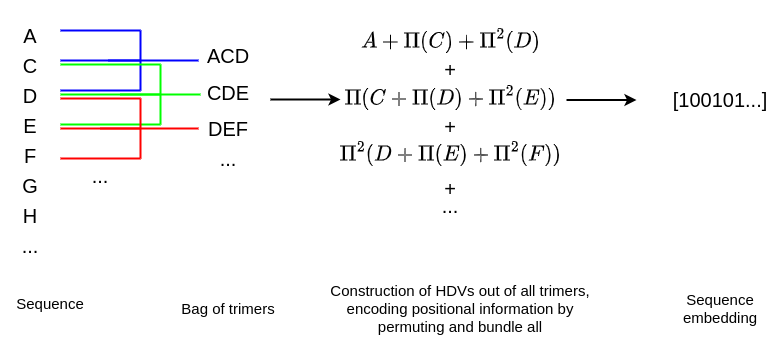
\includegraphics[scale = 0.6]{cnn.png}
    \caption{Overview of operations done to obtain an HDV from a sequence using the convolutional embedding method. First, a HDV is generated for every amino acid. Next, a peptide sequence is to be considered as a bag of trimers. A vector representing a trimer is generated by binding the three amino acids whilst retaining sequential information by shifting as in equation~\ref{eqn:trimer}, just as in the BoW-method (figure~\ref{fig:diagram_exprot}). On top of that, every trimer will also be positionally encoded via a permutation operation. All retrievable trimers from a given sequence are then bundled together, forming a hyperdimensional vector representative of the sequence.}
    \label{fig:cnn}
\end{figure}

These two sequence embedding methods have been applied to all sequences in the dataset using both random hyperdimensional vectors and extended ESM-2 embeddings. These were then visually assessed \textit{via} PCA.

\subsection*{Classification of hyperdimensional protein sequence embeddings}
As a baseline level, we use the rudimentary HDV classification technique as seen in chapter~\ref{sec:example}: the HDVs of sequences of the same class are bundled to construct single HDVs representative of every class. Then, a sequence's class is inferred by comparing the sequence's HDV to both class HDV \textit{via} a similarity measure based on the assumption that the class vector is maximally similar to its components. This model was evaluated \textit{via} a stratified 10-fold cross validation, trained and tested with all non-ML annotated proteins in the dataset. Out of the 11549 unambiguous UniParc accessions in the newest version of the database, 4829 are manually annotated on their type. Out of these manually annotated proteins, 2803 are endolysins and 2026 are VALs.

The baseline hyperdimensional classification model has been compared to a more established model, the XGBoost classifier~\cite{xgboost}. The classification with an XGBoost classifier is done via the default XGBoost classifier from \textit{XGBoost.jl v2.2.5} using the hyperdimensional embeddings as an input and is evaluated \textit{via} a stratified 10-fold cross validation with \textit{MLJ.jl v0.19.5}.

Another model we experimented with, is OnlineHD by A. Hernandez-Cano~\textit{et al.}~\cite{onlinehd}. It is an algorithm that expands on the classical hyperdimensional training methods by trying to eliminate model saturation. Instead of naively bundling vectors on top of each other, this algorithm assigns weights to every addition depending on how much new information it adds to the model to prevent class vector saturation. To train the model, assume a new data point $\vec{V}$ with label $l$ and class vectors $\vec{C_{i}}$ with each having a label $i$. The cosine similarity of $\vec{V}$ with every class vector is then calculated as $cos_{i}$. If $\vec{V}$ with an actual label $l$ would have been predicted as $l'$, the class vectors will be updated as followed (with learning rate $\eta$):

\begin{alignat}{1}
    \label{eqn:onlinehd}
    \vec{C_{l}} &\leftarrow \vec{C_{l}} + \eta (1 - cos_{l}) * \vec{V} \\
    \vec{C_{l'}} &\leftarrow \vec{C_{l'}} - \eta (1 - cos_{l'}) * \vec{V}
\end{alignat}

This means that if a new data point is highly dissimilar to its class vector and thus contains a high amount of new information, the weight of the update ($\eta (1 - cos_{l})$) will increase. The information is then also subtracted from the incorrectly predicted class vector. If a label would be correctly predicted for a new data point, the model will not be updated to avoid saturation. To initialize the model, the first vector of a class to be assessed is assumed to be the class vector. For example, if a query vector in our dataset is predicted to be a VAL, but its actual label is endolysin, the class vectors are then updated as followed:

\begin{alignat}{1}
    \label{eqn:onlinehd2}
    \vec{C_{VAL}} &\leftarrow \vec{C_{VAL}} + \eta (1 - cos_{VAL}) * \vec{V} \\
    \vec{C_{endo}} &\leftarrow \vec{C_{endo}} - \eta (1 - cos_{endo}) * \vec{V}
\end{alignat}

Due to the nature of this model, we cannot constrict our hyperdimensional embeddings to a bipolar or binary nature anymore and the embeddings are then allowed to be real-numbered. Mathematical operations such as multiplications and additions are then assumed to be element-wise. On top of the single-pass method as discussed above, A. Hernandez-Cano~\textit{et al.} also implemented an iterative retraining algorithm to increase the accuracy of OnlineHD. This starts from the class vectors made \textit{via} the single-pass OnlineHD model, but assesses the class vectors by performing inference with every training vector. If a training vector's label is wrongly predicted, equations 4.1 and 4.2 are then used to update the model. This entire sequence is iterated over a given amount of cycles.

Since these algorithms are only available as \textit{PyTorch} implementations, implementations in \textit{Julia} have been made here. A stratified 10-fold cross validation of these models with our subject sequences has been performed. The learning rate is set at 0.035 and the amount of retraining iterations is set to 120. To test these algorithms, real-numbered embeddings had to be made from our subject sequences. So instead of embedding the sequences starting with random bitvectors, random vectors with values in interval $[-1, 1]$ for both the random amino acid vectors and extended ESM-2 embeddings were made to obtain real-valued hyperdimensional vectors for every amino acid. The same bag-of-words and convolutional approaches have been applied here to obtain sequence embeddings. These embeddings were assessed \textit{via} a scatter-plot of the two first principal components of their PCA projection.
\section{Results}
\subsection*{Embedding of sequences into hyperdimensional vectors}
There is no visual difference between the PCA plots for the sequences embedded \textit{via} the bag-of-words method and the convolutional method, but there is a clear difference between the different starting embeddings as seen in figure 4.2. The sequence embeddings from both the bag-of-words method and the convolutional method made with ESM-2 AA embeddings seem to capture more of the variance between the sequences.

\begin{figure}[H]
    \centering
    \begin{subfigure}[b]{0.4\textwidth}
        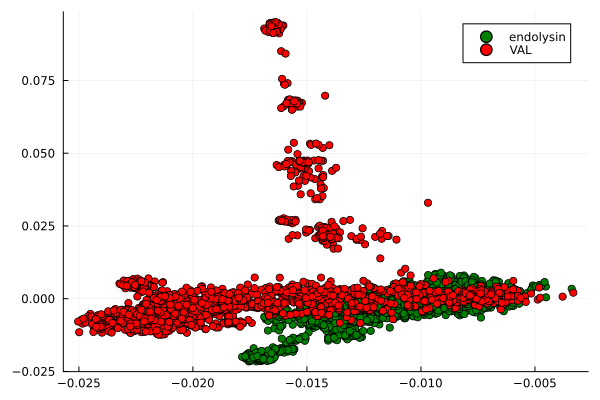
\includegraphics[width=\textwidth]{phalp_bow_rand}
        \caption{BoW-encoded protein sequences, starting from random vectors. These PCs account for roughly 7 \% of the total variance in the system.}
    \label{fig:phalpbowrand}
    \end{subfigure}
        \hspace{1cm}
    \begin{subfigure}[b]{0.4\textwidth}
        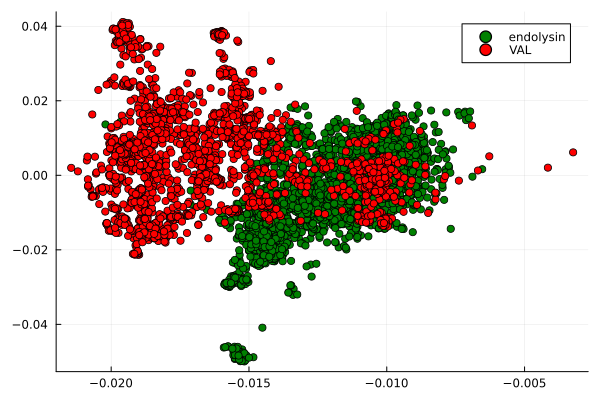
\includegraphics[width=\textwidth]{phalp_bow_esm}
        \caption{BoW-encoded protein sequences, starting from extended ESM-2 embeddings. These PCs account for roughly 15.5 \% of the total variance in the system.}
    \label{fig:phalpbowesm}
    \end{subfigure}
    \label{fig:phalp_emb}
    \caption{Scatter-plot of the first two principal components of the binary encoded phage lytic proteins \textit{via} the BoW-method starting from (a) random HDVs per amino acid (b) extended ESM-2 embeddings. Only manually annotated phage lytic proteins were considered and are color-coded based on their type.}
\end{figure}
\subsection*{Classification of hyperdimensional protein sequence embeddings}
Evaluating our naive additive model using stratified 10-fold cross-validation results in F1-scores of around 0.14 for every kind of hyperdimensional embedding as seen in table~\ref{tab:phalpclass}. This low result is likely due to the possibility of oversaturation of the class vectors.

THIS PART MAYBE IN DISCUSSION IF THAT WILL BE SEPERATE? We can predict the angle between a class vector and a randomly selected vector from said class by $\Theta = \arccos({2k \choose k}/2^{2k})$ with $2k+1$ equal to the number of sequences in the class~\cite{sathdv}. This approximation is valid for bipolar vectors in hyperdimensions $(\ge 10000)$. This equation also suggests that an increase in dimensions will not influence the angle. Evaluating this equation by considering random 1001 vectors in a class, so $k = 500$, results in an angle of $88.6^{\circ}$. This indicates that a vector has a limited capacity: the more vectors we bundle together, the closer the angle will be to $90^{\circ}$ and thus the more dissimilar the class vector becomes to its components. This results in the class vectors not being representative anymore of a given dataset. This equation assumes that the class vector is a bundle of purely random vectors which is not the case for our embeddings; however, it provides us a rough idea about the bundling capacity of a hyperdimensional vector. Thus, using the rudimentary model works only for very small datasets, as seen in the examples in chapter~\ref{sec:example}. So to encode larger datasets, the training algorithm has to be more refined.

\begin{table}[h]
    \caption{\label{tab:phalpclass}Results of type classifications using the principal classification technique of hyperdimensional computing,an XGBoost classifier and OnlineHD implementations with several kinds of embeddings}
    \resizebox{\textwidth}{!}{\begin{tabular}{|c||c|c|c|c|}
        \hline
        \underline{F1-scores} & \textbf{BoW/random} & \textbf{BoW/ESM} & \textbf{Convolutional/random} & \textbf{Convolutional/ESM} \\
        \hline
        \textbf{Naive addition} & 0.1458 & 0.1468 & 0.1461 & 0.1461 \\
        \hline
        \textbf{XGBoost classifier} & 0.9667 & 0.9754 & 0.9661 & 0.986 \\
        \hline
        \textbf{Single-pass OnlineHD} & 0.8901 & 0.9214 & 0.7793 & 0.8400 \\
        \hline
        \textbf{Iterative OnlineHD} & 0.9487 & 0.9757 & 0.9486 & 0.9670 \\
        \hline
    \end{tabular}}
\end{table}

The results of the XGBoost classifer for the same embeddings are much more comparable to the results of the experiment in the PhaLP paper with the convolutional embeddings generally performing better than the bag-of-words embeddings and also the ESM-based embeddings performing better than random base vectors. This is an indication that hyperdimensional computing can provide a very fast and reliable method of embedding protein sequences, even without prior biological information. The drawback of this machine learning model, which is to be expected from every gradient-based model, is that training and predictions take much longer to compute compared to hyperdimensional training models. The cross validation procedure took up to 5 minutes on a consumer-grade laptop, whilst with the naive additive approach, the procedure took less than 10 seconds to finish.

Comparing the results of the OnlineHD models to the naive additive HDC model, we can see a substantial increase in the performance of this model. The single-pass model seems to have more widely varying results depending on the type of embeddings used. As opposed to the XGBoost classifier, it performs better using bag-of-words embeddings. The model also performs better when trained with embeddings based on extended ESM-2 vectors. Iterative retraining of the model seems to increase its performance significantly, even coming close to the performance of an XGBoost classifier in this case. Further improvement might be found when optimizing the models' parameters. The cross validation procedure takes less than 10 seconds to run for the single-pass model, whilst doing an iterative retraining of the model adds 2 to 3 minutes. This model appears to be a decently performing extension of the rudimentary hyperdimensional classification model for protein classification, whilst still being much more efficient than the commonly used machine learning models. The drawback of the model is that we cannot use hyperefficient bit-operations anymore, which limits its efficiency compared to the binary nature of the additive model.

\begin{figure}[h!]
    \centering
    \begin{subfigure}{0.48\textwidth}
        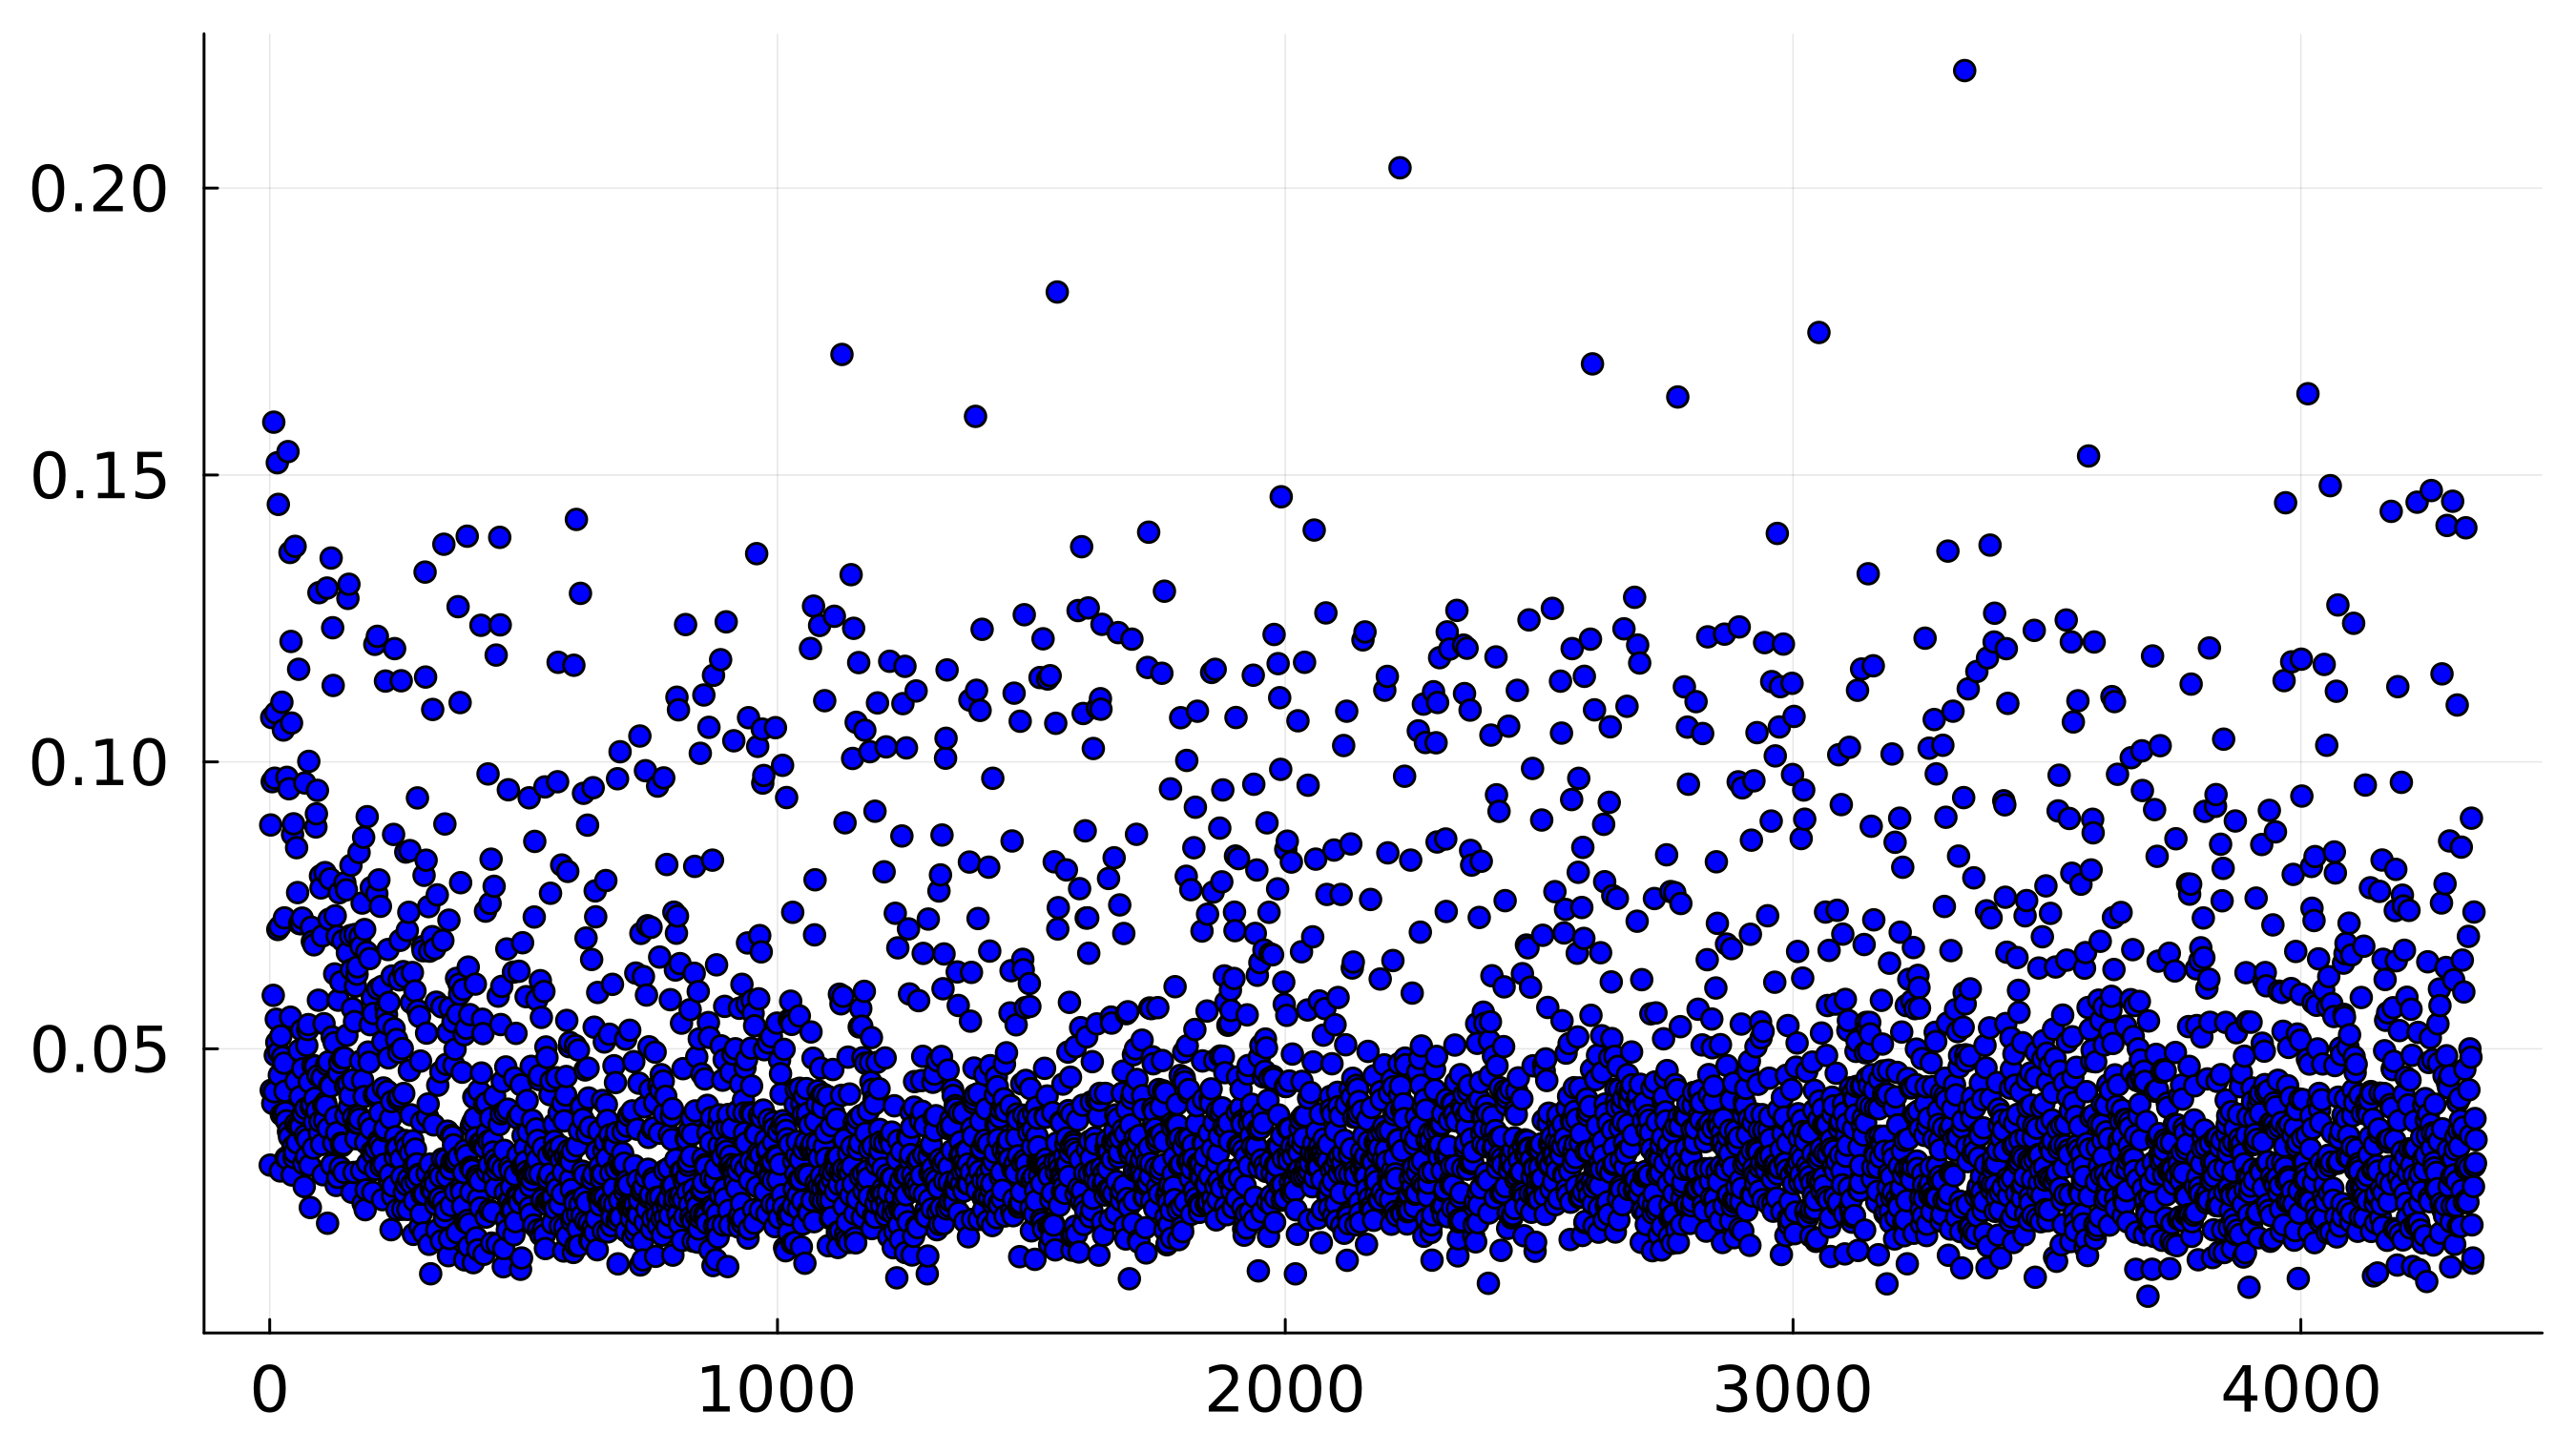
\includegraphics[width=\textwidth]{phalp_bow_rand_learning3}
        \caption{Embeddings using random amino acid vectors, made \textit{via} the bag-of-words embedding method}
        \label{fig:subfig-a2}
    \end{subfigure}
    \hfill
    \begin{subfigure}{0.48\textwidth}
        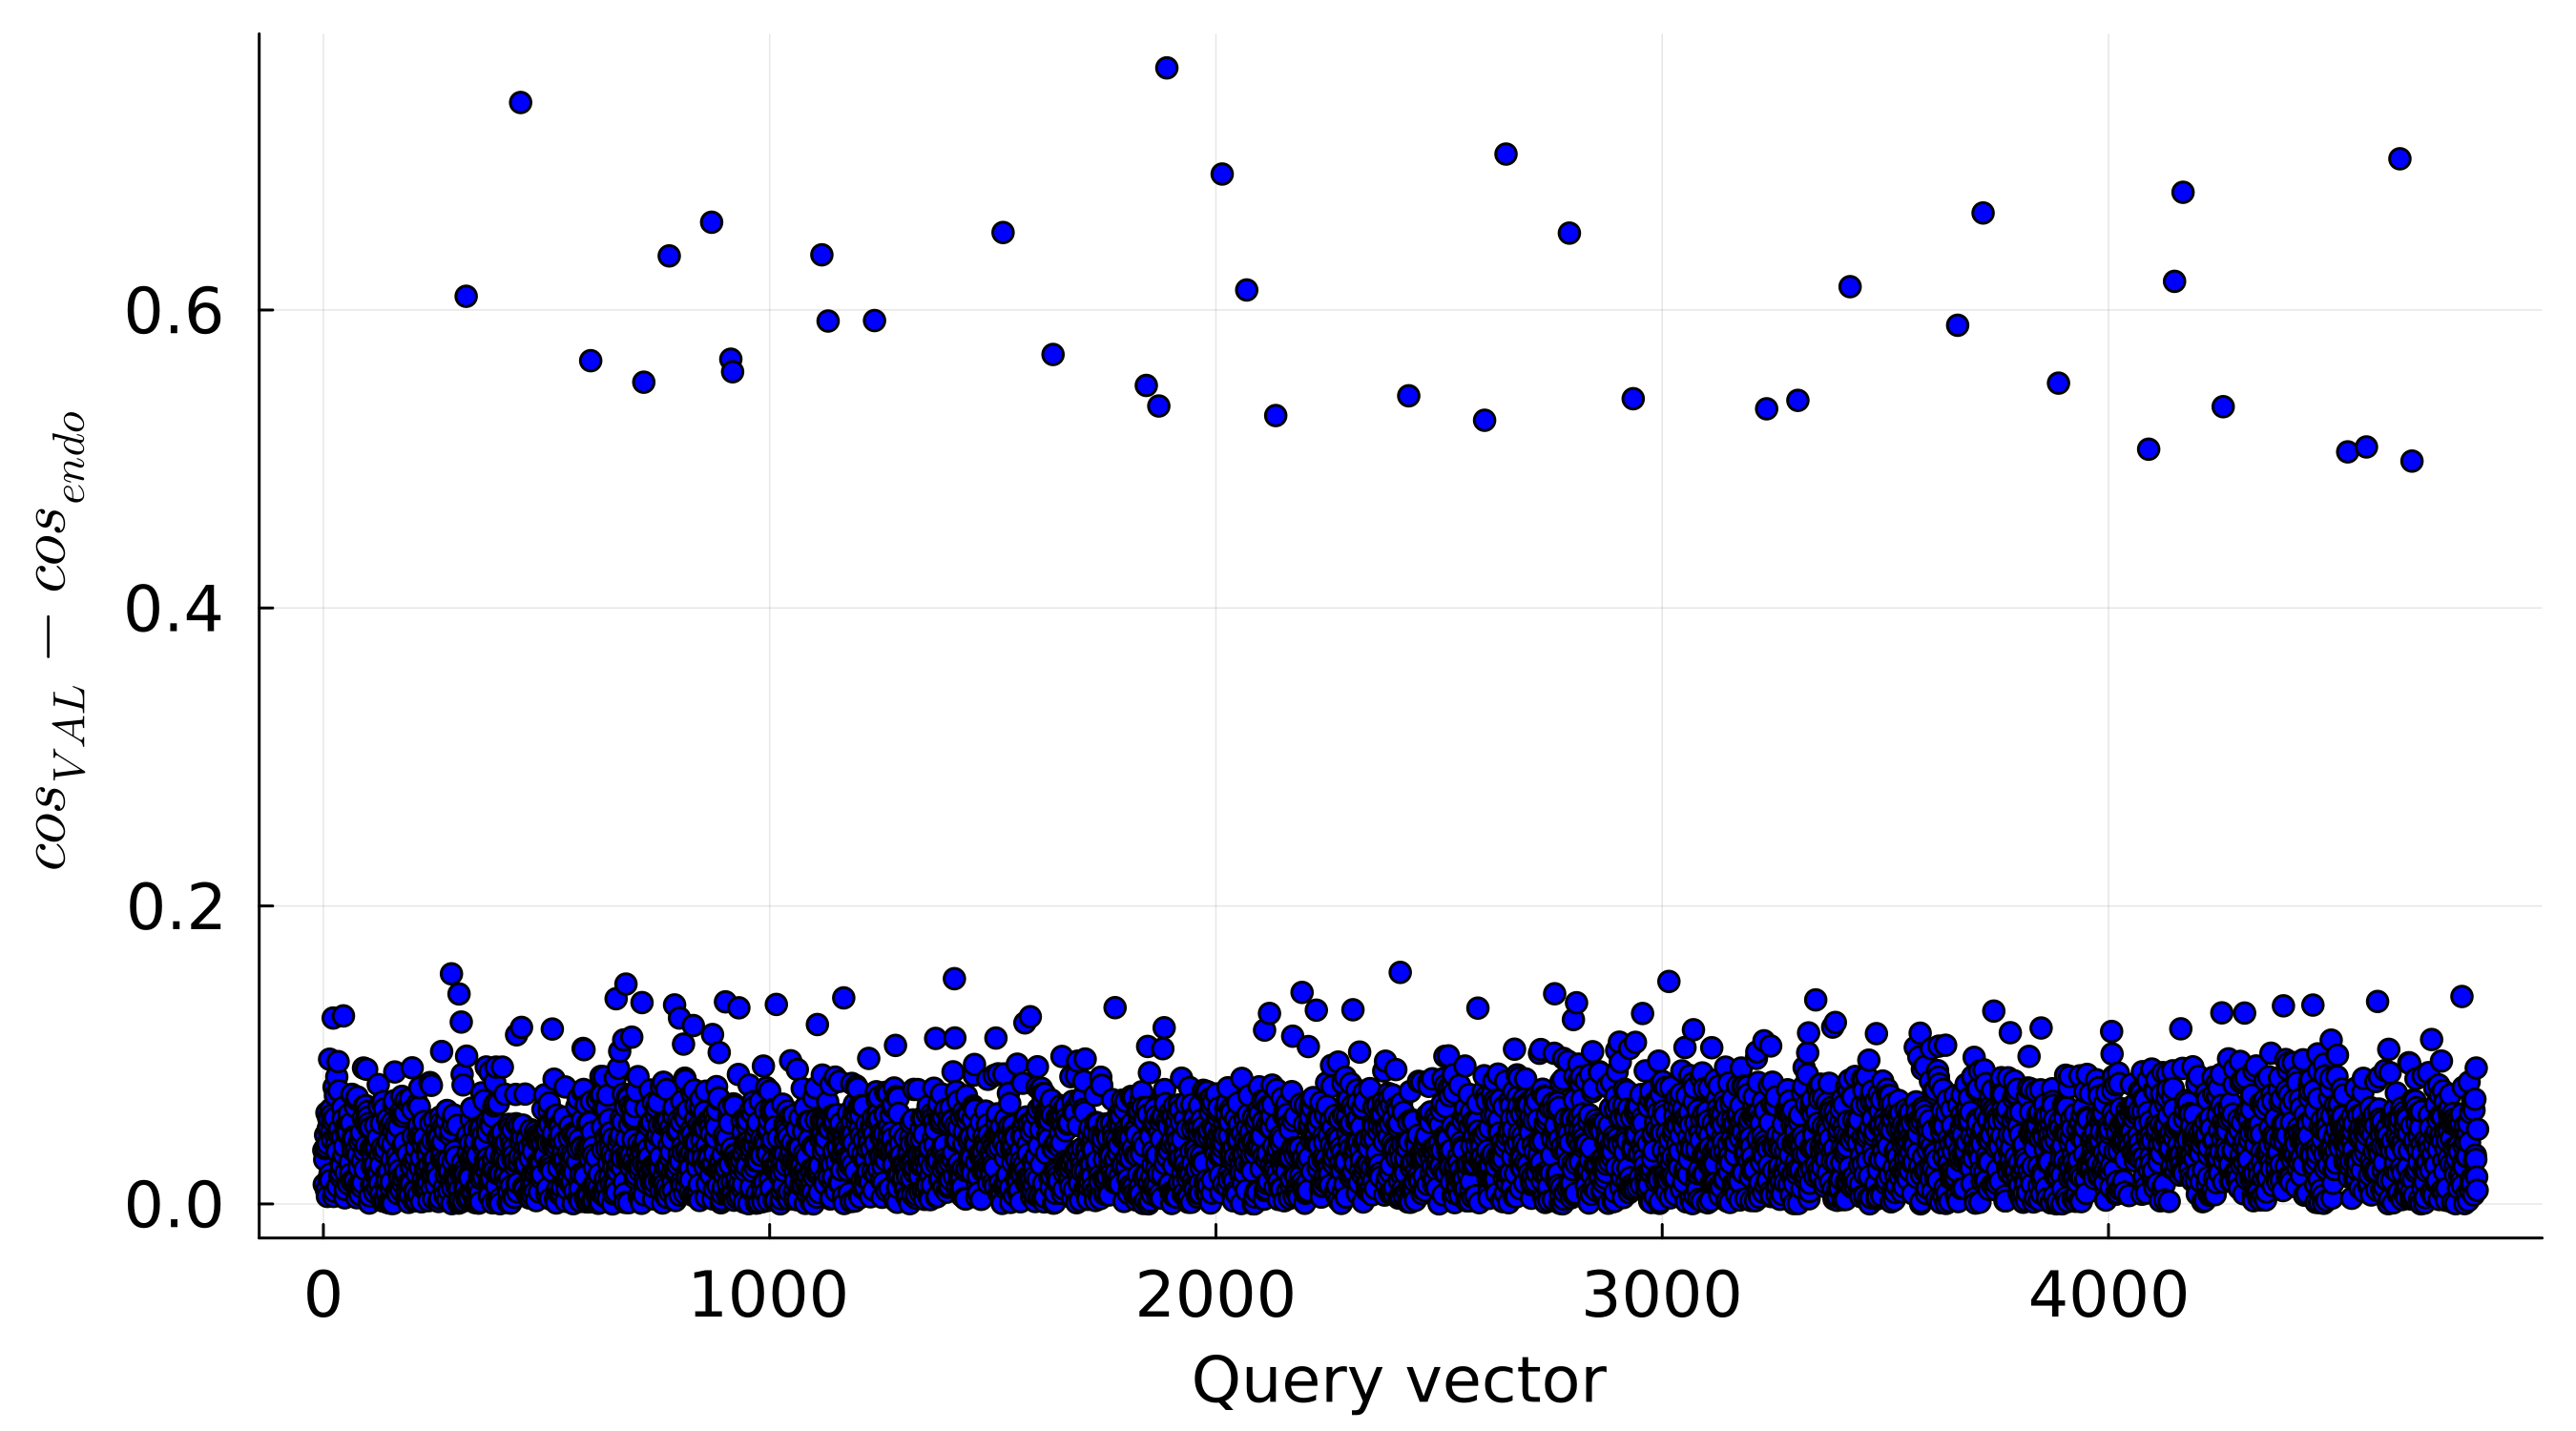
\includegraphics[width=\textwidth]{phalp_bow_esm_learning3}
        \caption{Embeddings using extended ESM-2 amino acid vectors, made \textit{via} the bag-of-words embedding method}
        \label{fig:subfig-b2}
    \end{subfigure}
    
    \begin{subfigure}{0.48\textwidth}
        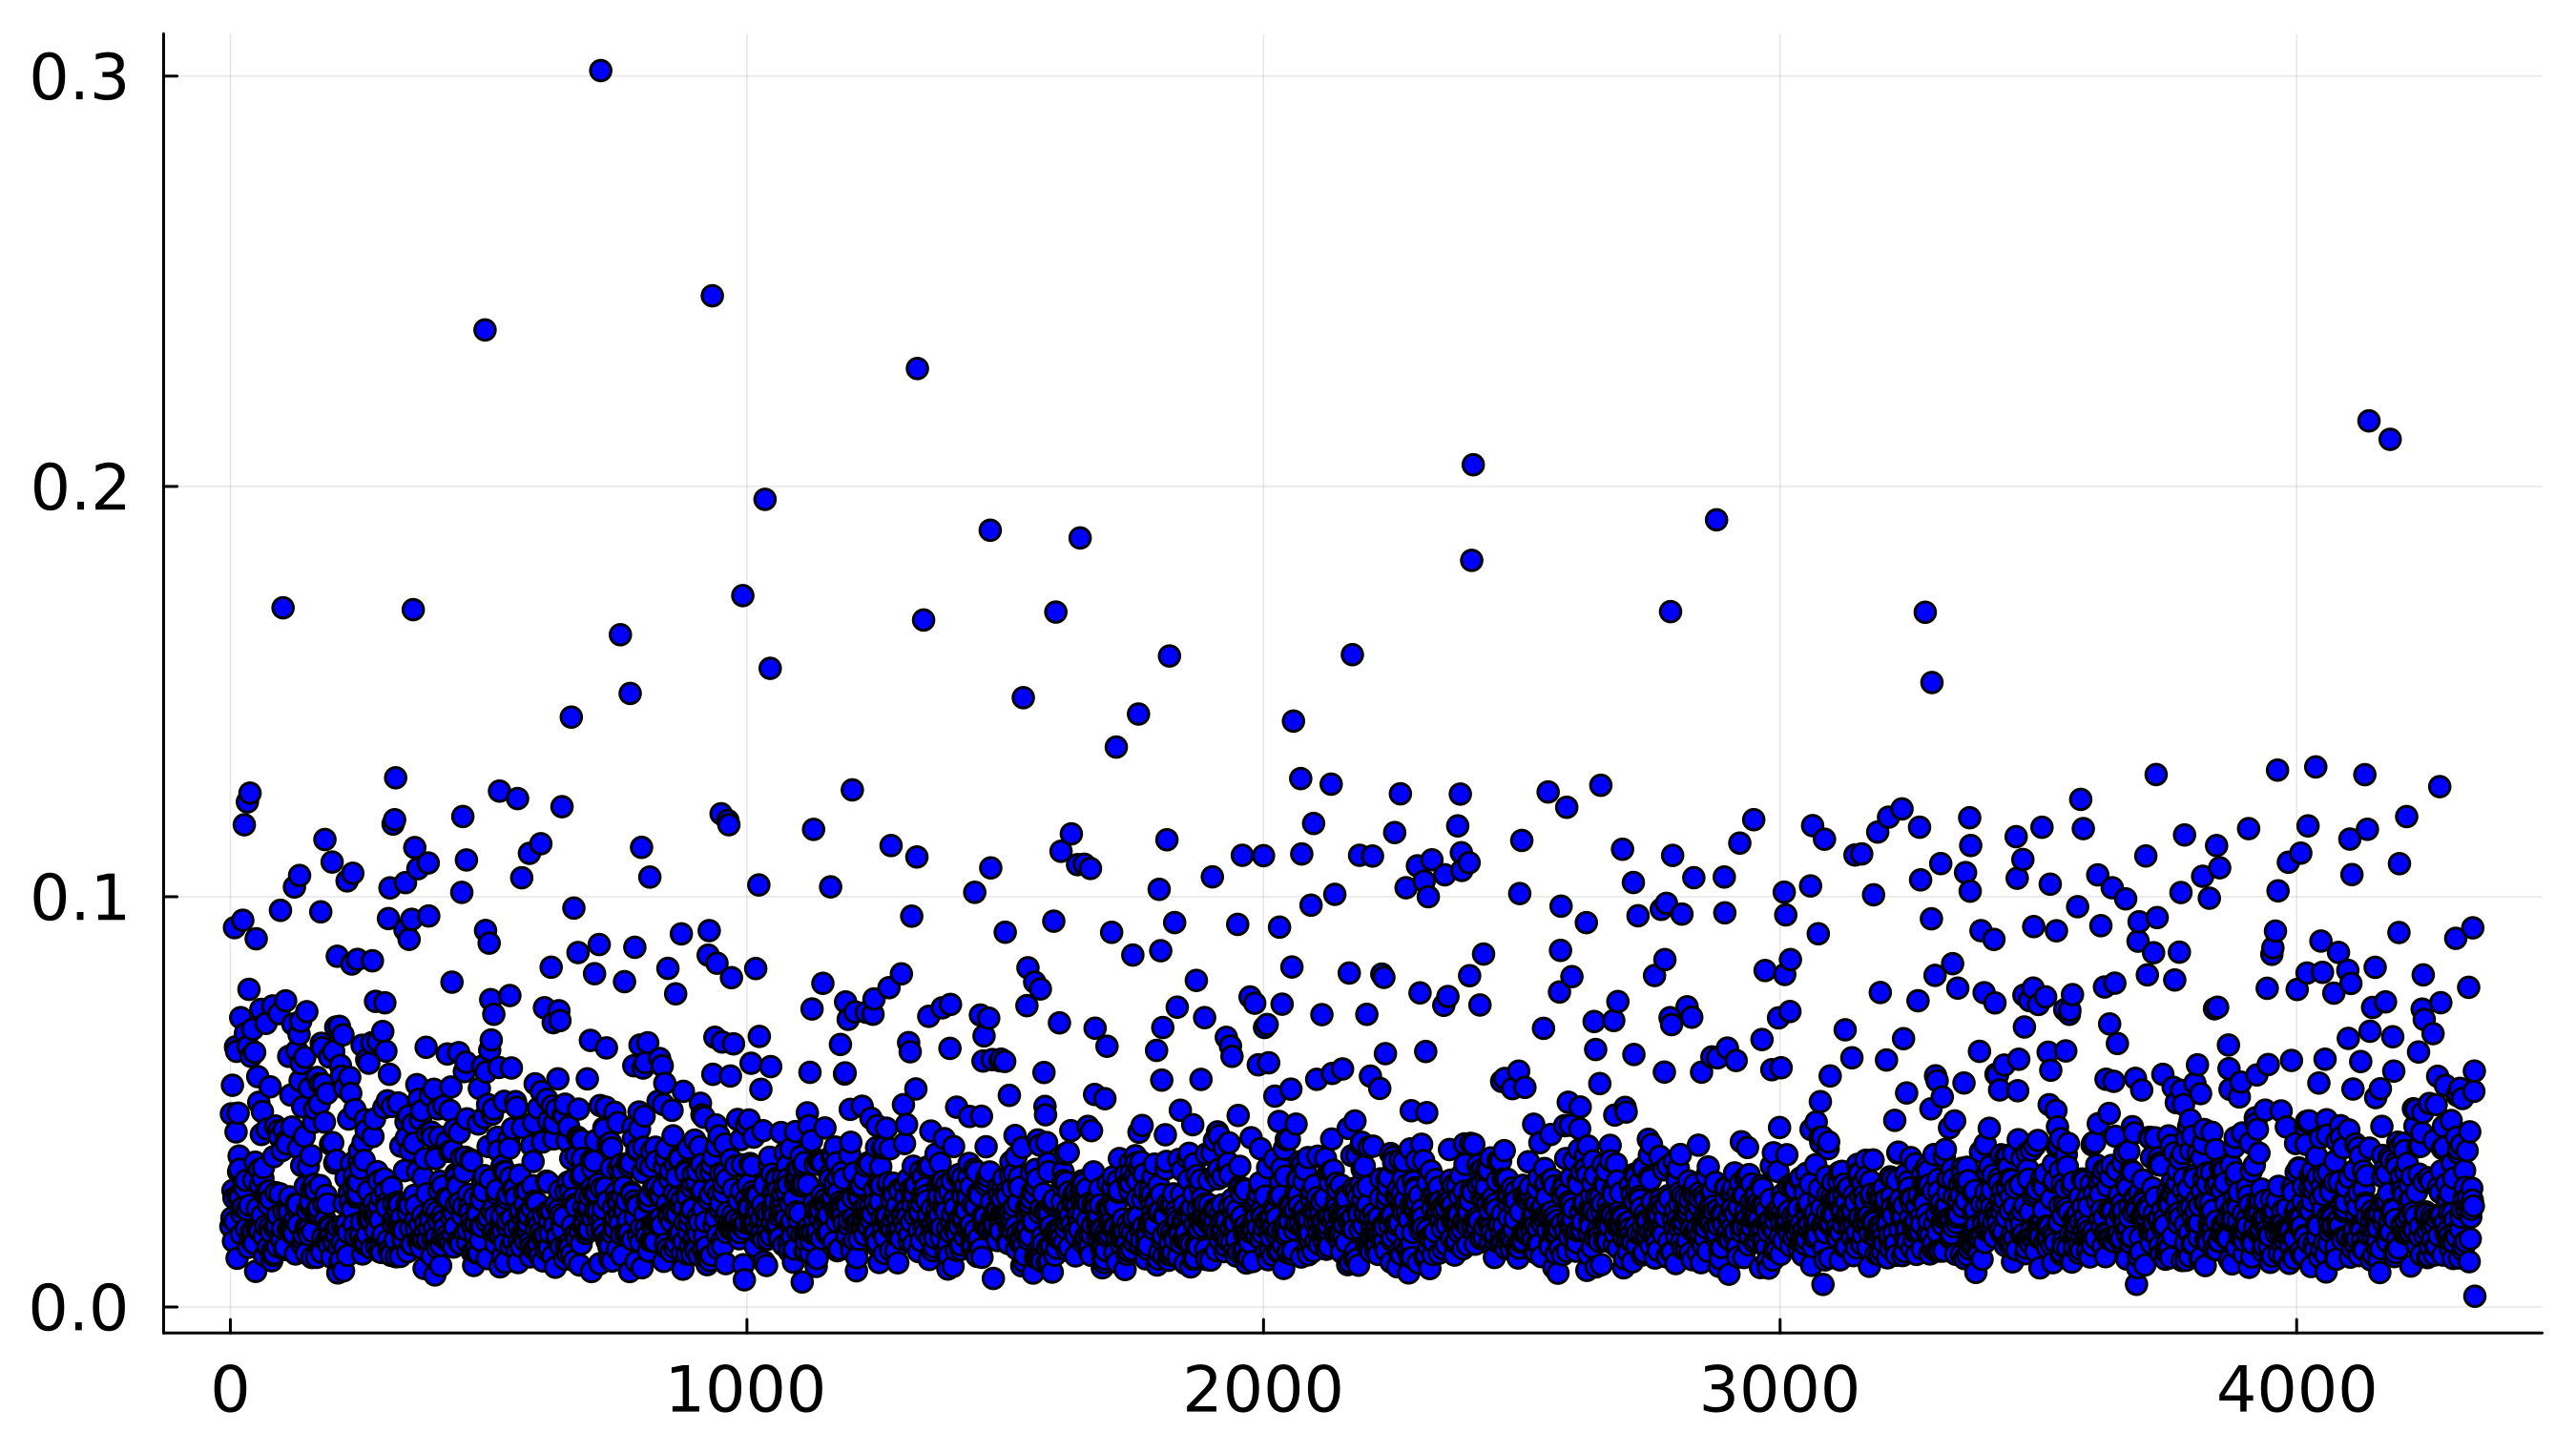
\includegraphics[width=\textwidth]{phalp_cnn_rand_learning3}
        \caption{Embeddings using random amino acid vectors, made \textit{via} the convolutional embedding method}
        \label{fig:subfig-c2}
    \end{subfigure}
    \hfill
    \begin{subfigure}{0.48\textwidth}
        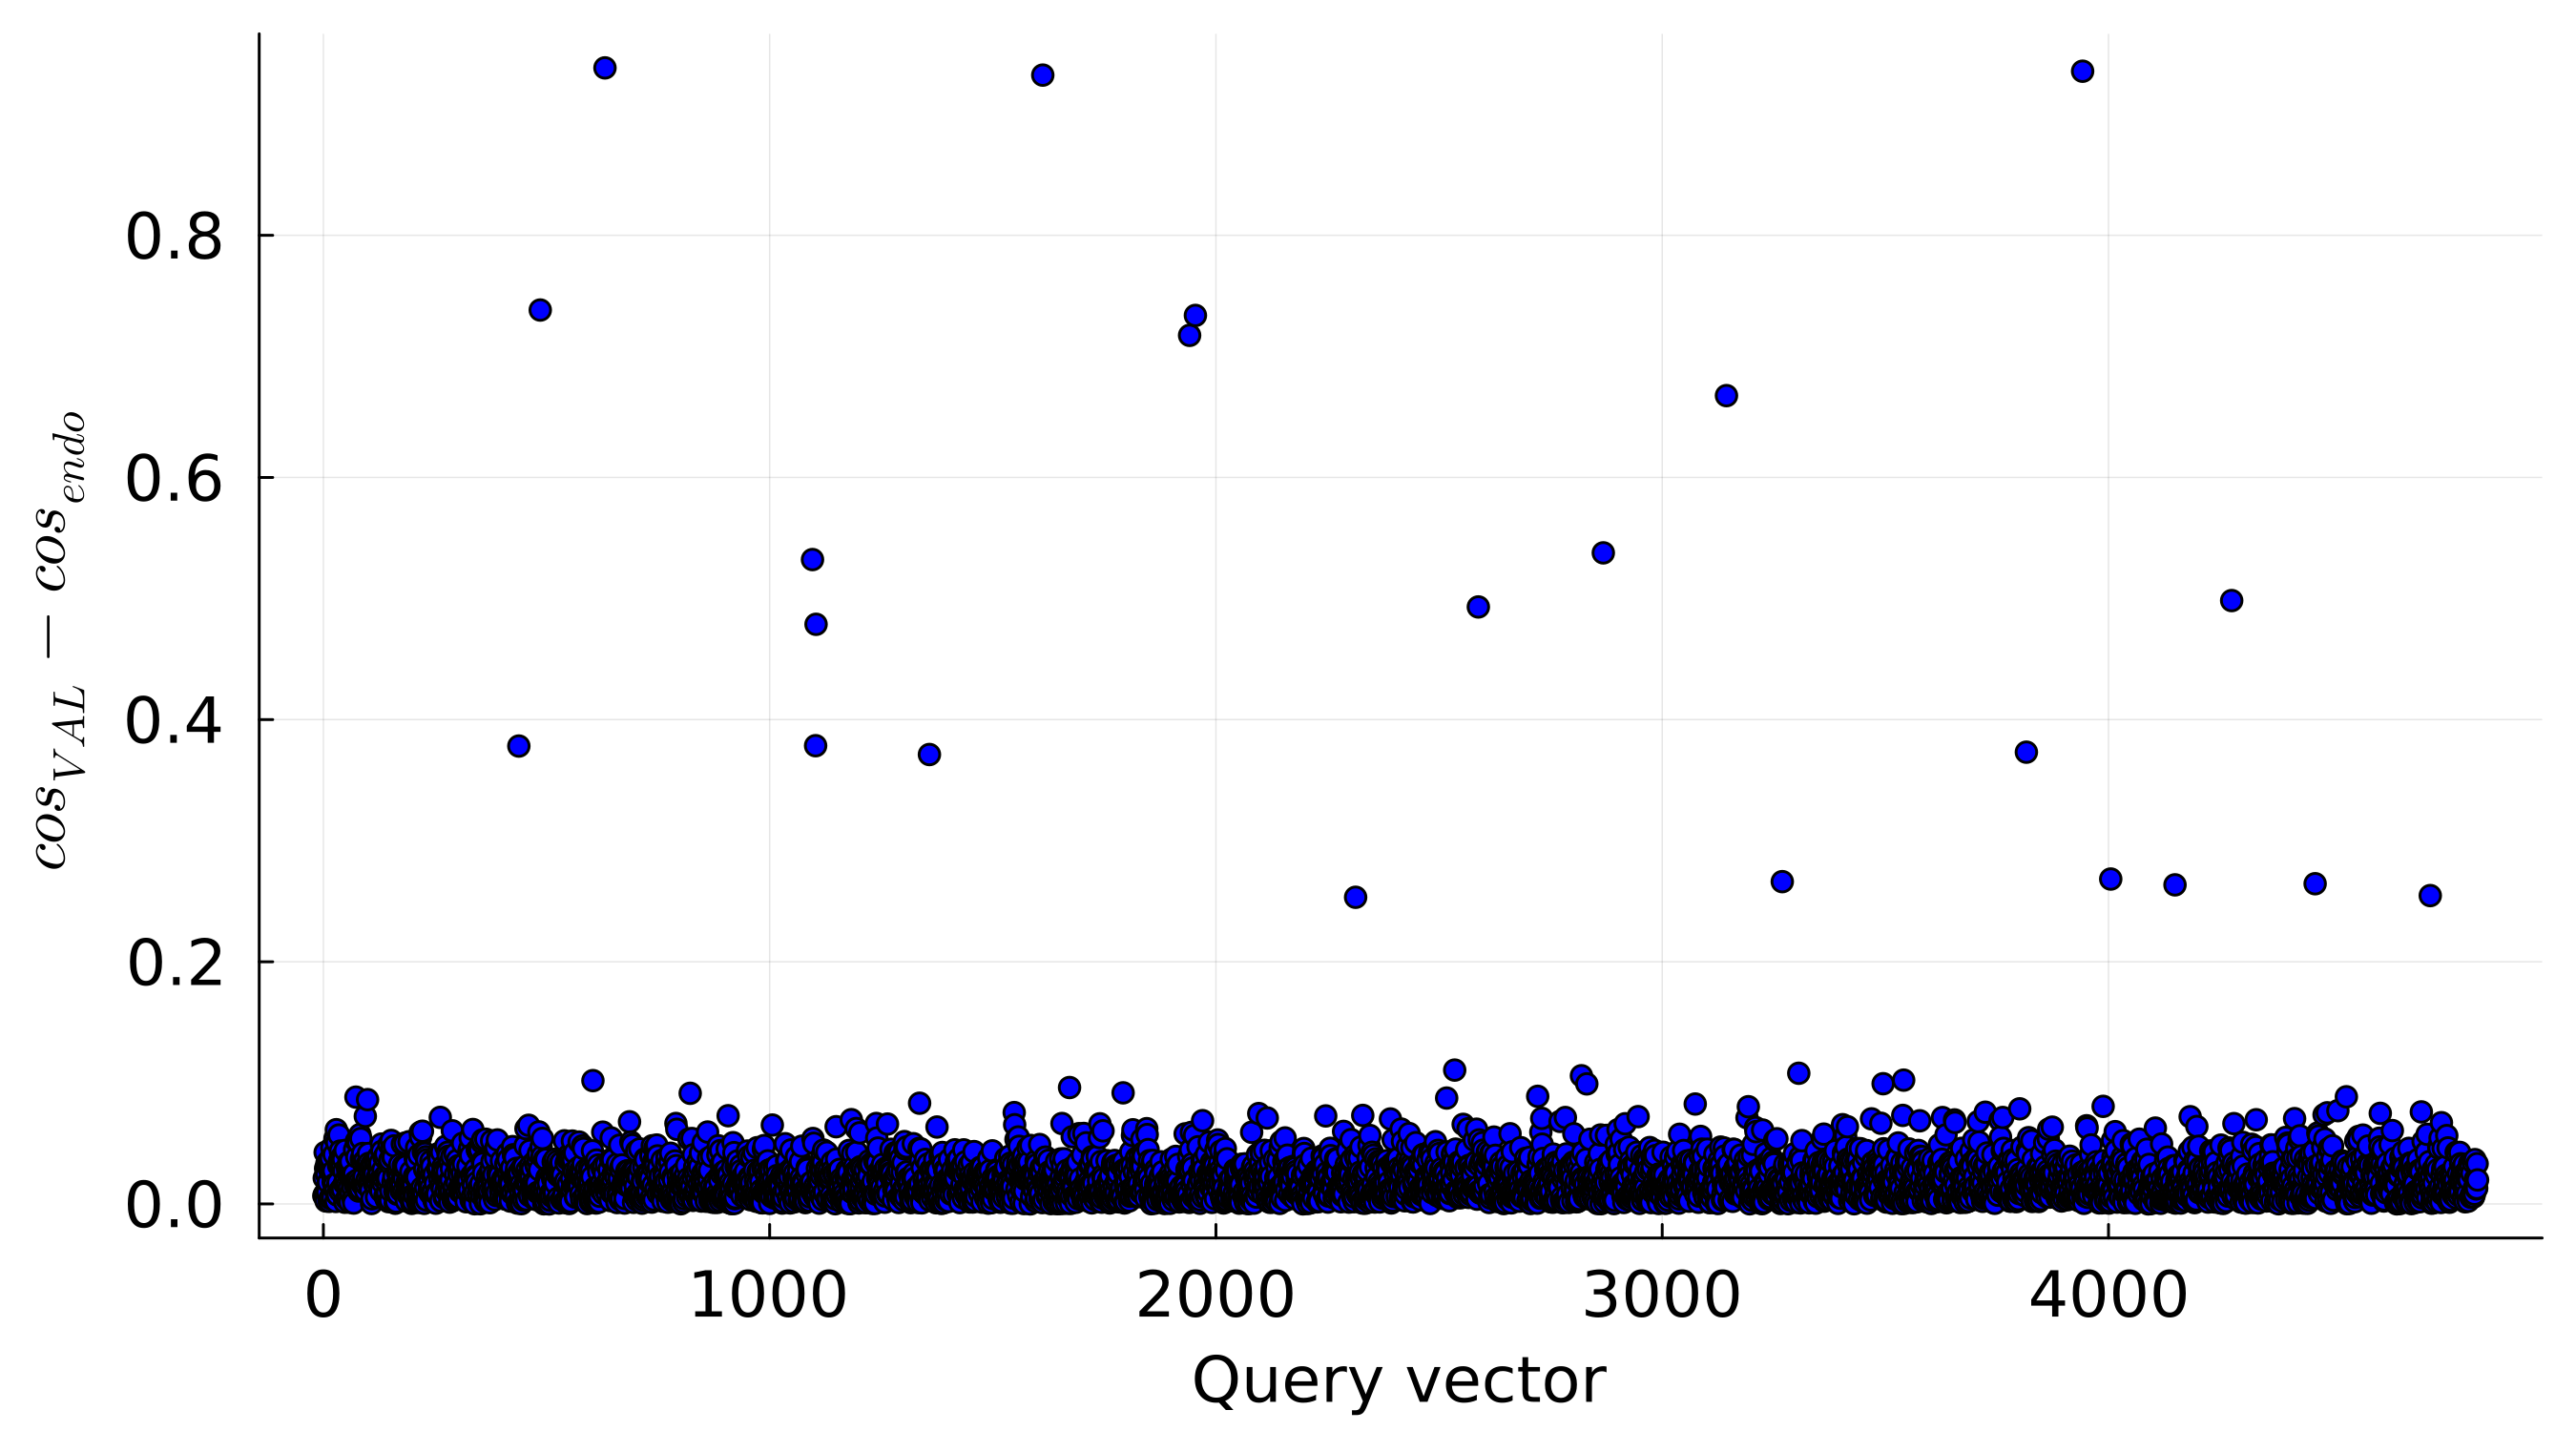
\includegraphics[width=\textwidth]{phalp_cnn_esm_learning3}
        \caption{Embeddings using extended ESM-2 acid vectors, made \textit{via} the convolutional embedding method}
        \label{fig:subfig-d2}
    \end{subfigure}
    \caption{Absolute difference between the cosine similarity of the query vector with the VAL class vector and the cosine similarity of the query vector with the endolysin class vector, averaged across the 10 cross validations while following the OnlineHD single-pass training procedure. Trained using hyperdimensional embeddings from all protein sequences in the PhaLP dataset whose types were manually annotated.}
    \label{fig:main2}
\end{figure}

In figure~\ref{fig:main2}, we aim to monitor the training process of the OnlineHD single-pass model when applied to the PhaLP dataset. To track the training progress, we calculate the absolute difference between the cosine similarities, $cos_{VAL}$ and $cos_{endo}$, as described in equations 4.3 and 4.4. These differences are averaged across all 10 cross-validation folds. By observing this metric, we can gain insights into the behavior of the hyperdimensional vectors in the OnlineHD model during training. we expect the difference in cosine similarities to increase throughout the training procedure as the model learns to differentiate the two classes. However, these differences don't increase noticeably increase in this case.

\begin{figure}[htbp]
    \centering
    \begin{subfigure}{0.48\textwidth}
        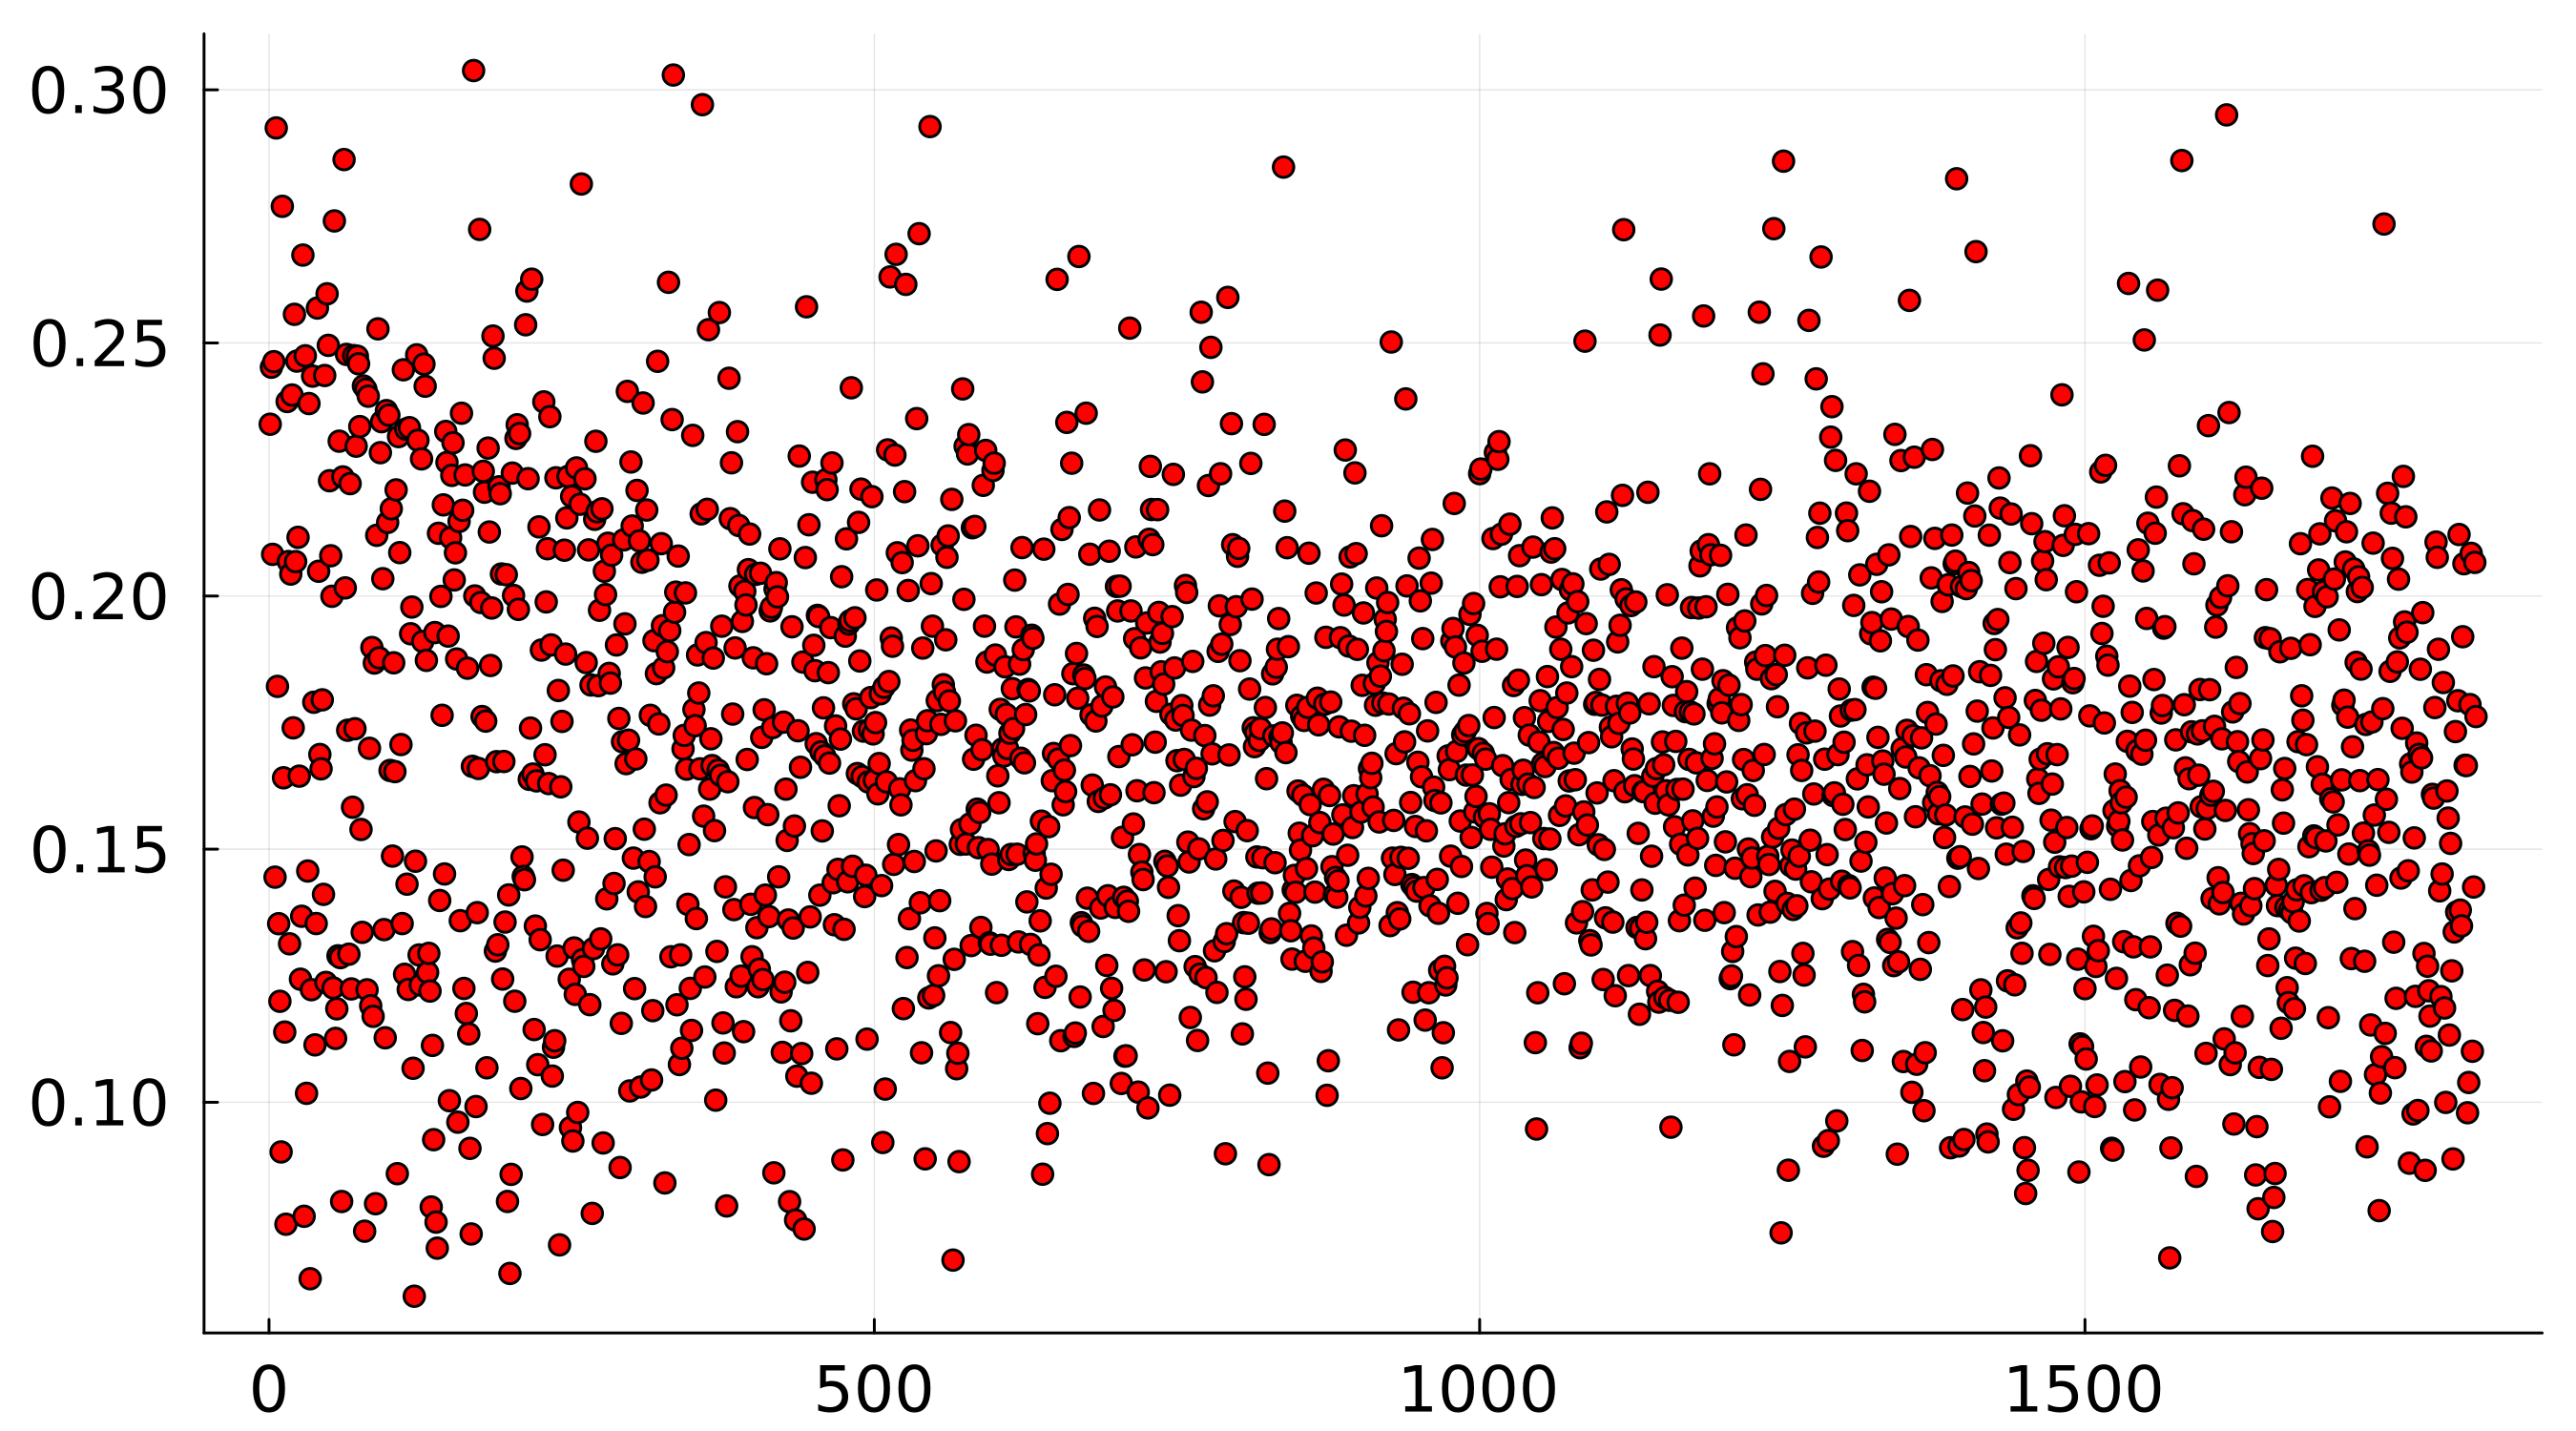
\includegraphics[width=\textwidth]{phalp_bow_rand_learningV}
        \caption{VALs embedded using random amino acid vectors \textit{via} the bag-of-words method}
        \label{fig:subfig-a}
    \end{subfigure}
    \hfill
    \begin{subfigure}{0.48\textwidth}
        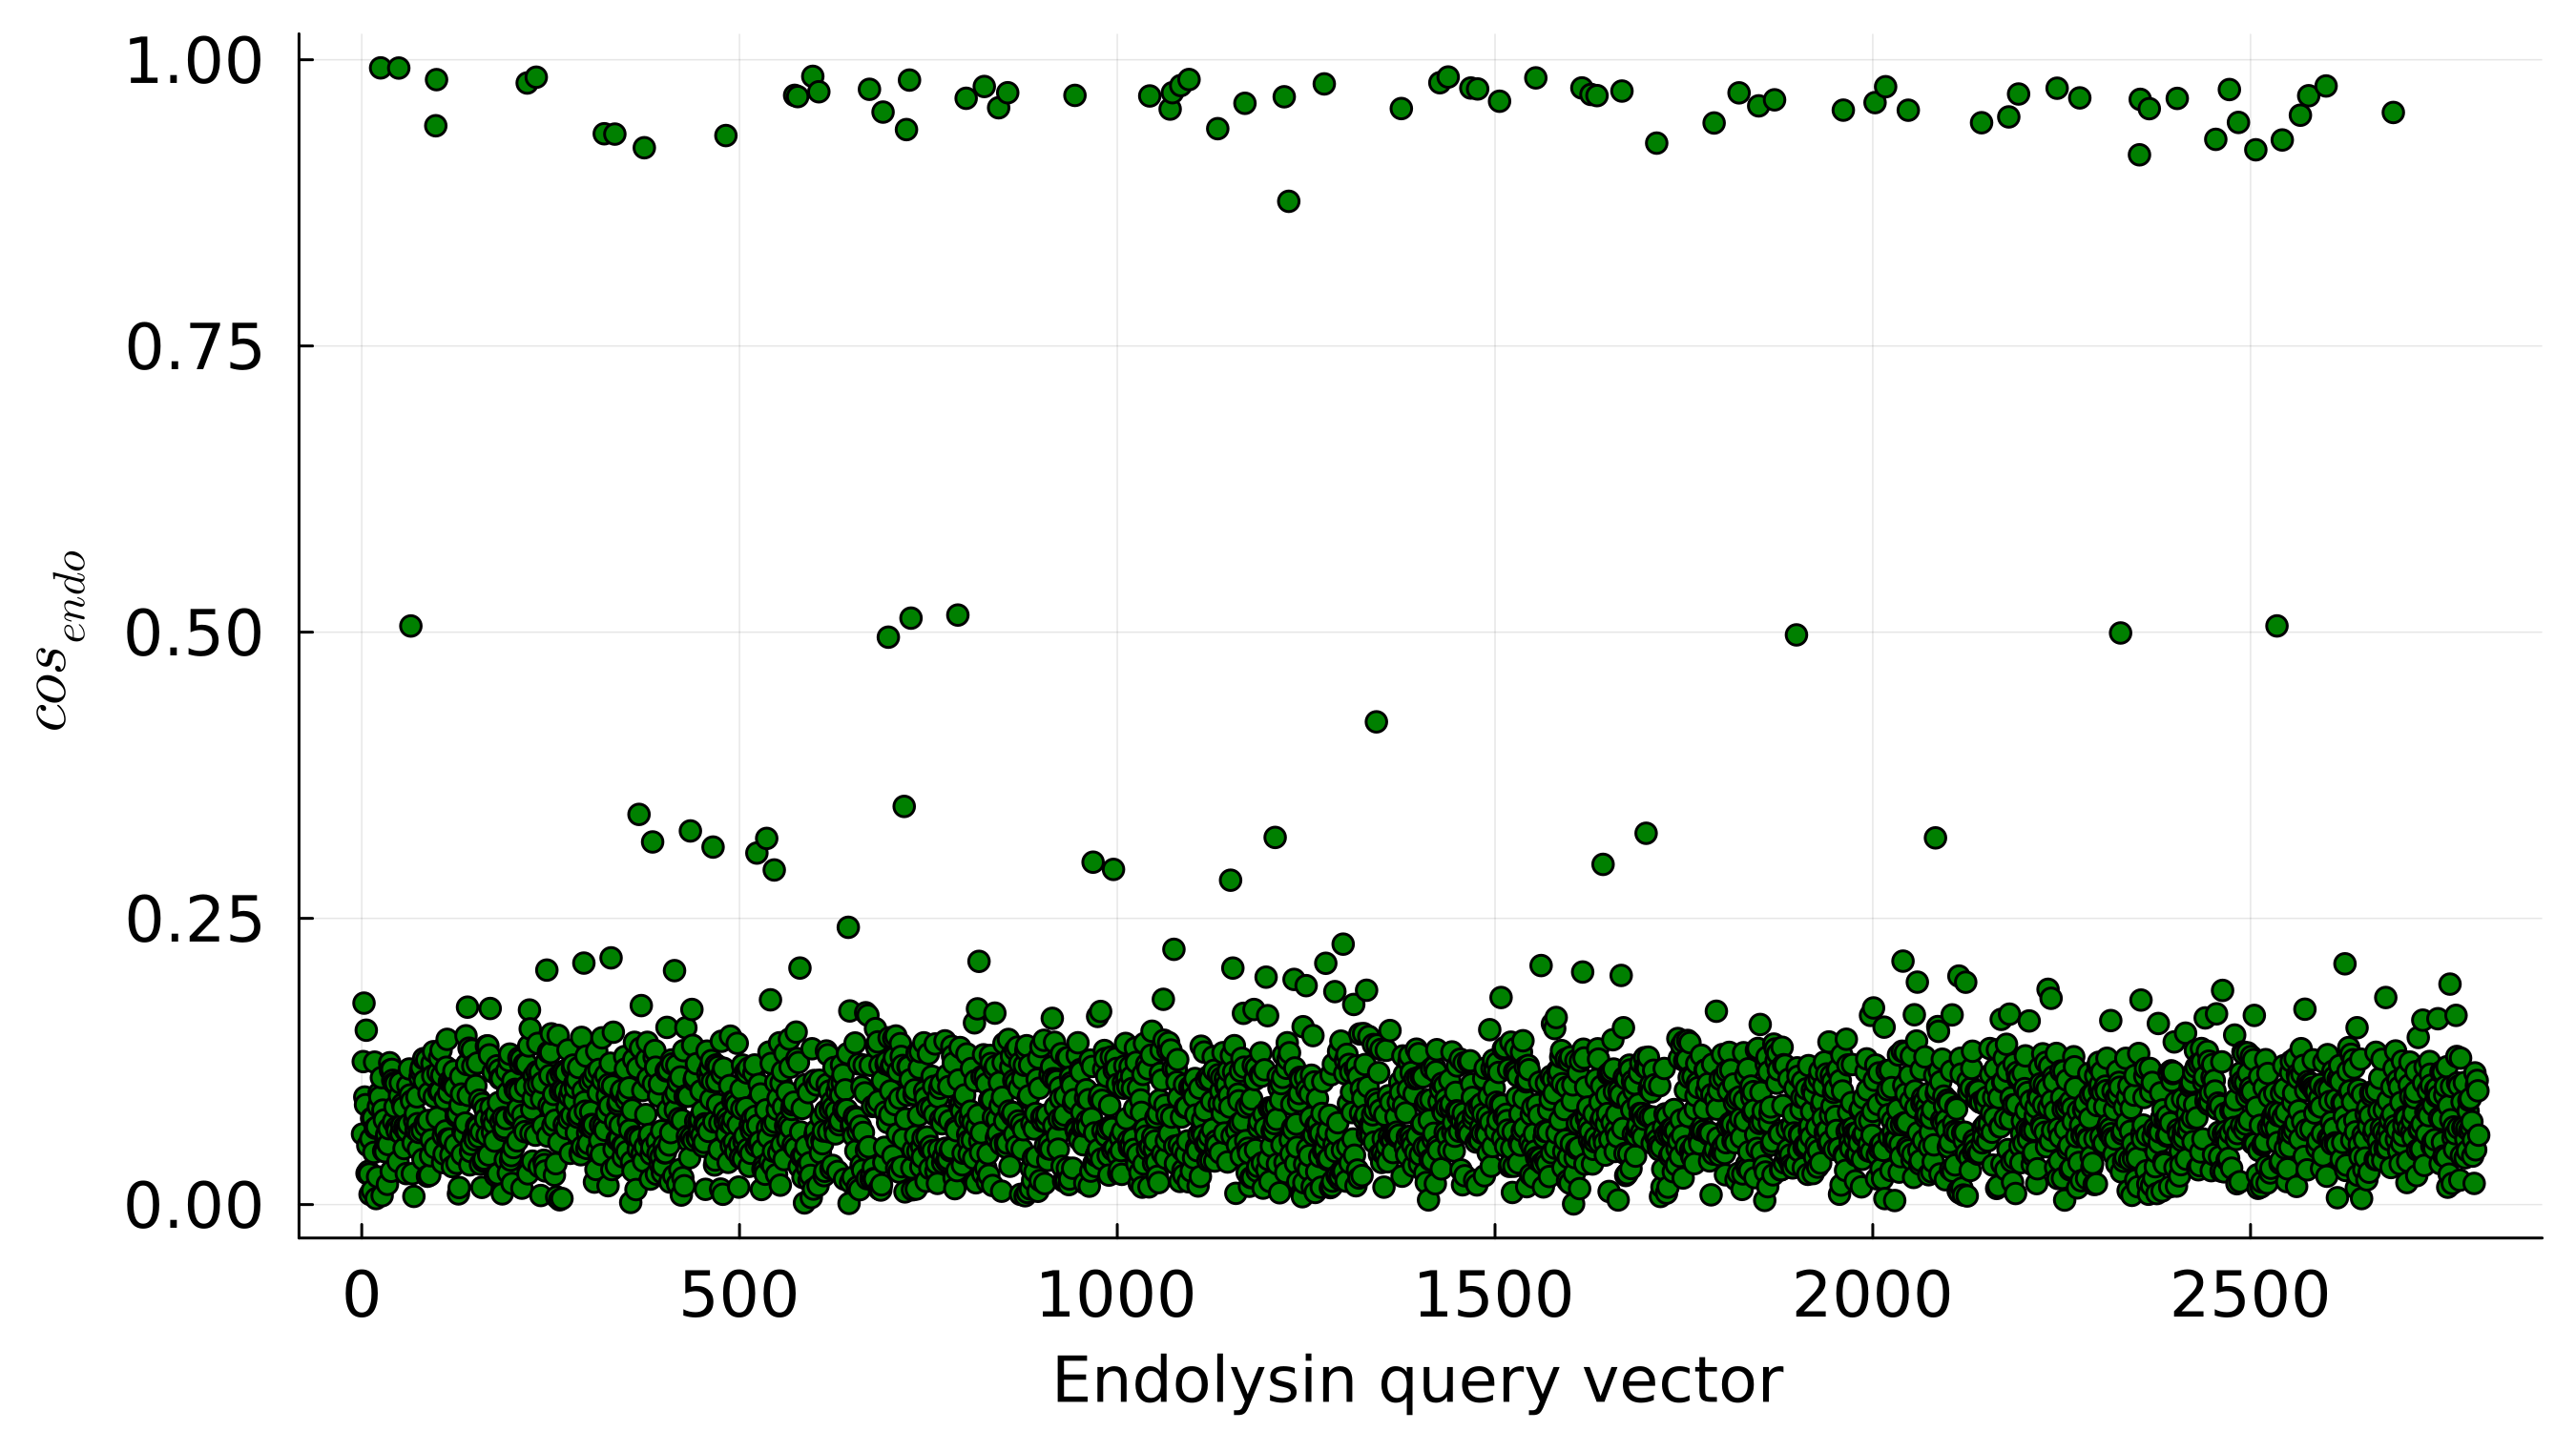
\includegraphics[width=\textwidth]{phalp_bow_rand_learningE}
        \caption{Endolysins embedded using random amino acid vectors \textit{via} the bag-of-words embedding method}
        \label{fig:subfig-b}
    \end{subfigure}
    
    \begin{subfigure}{0.48\textwidth}
        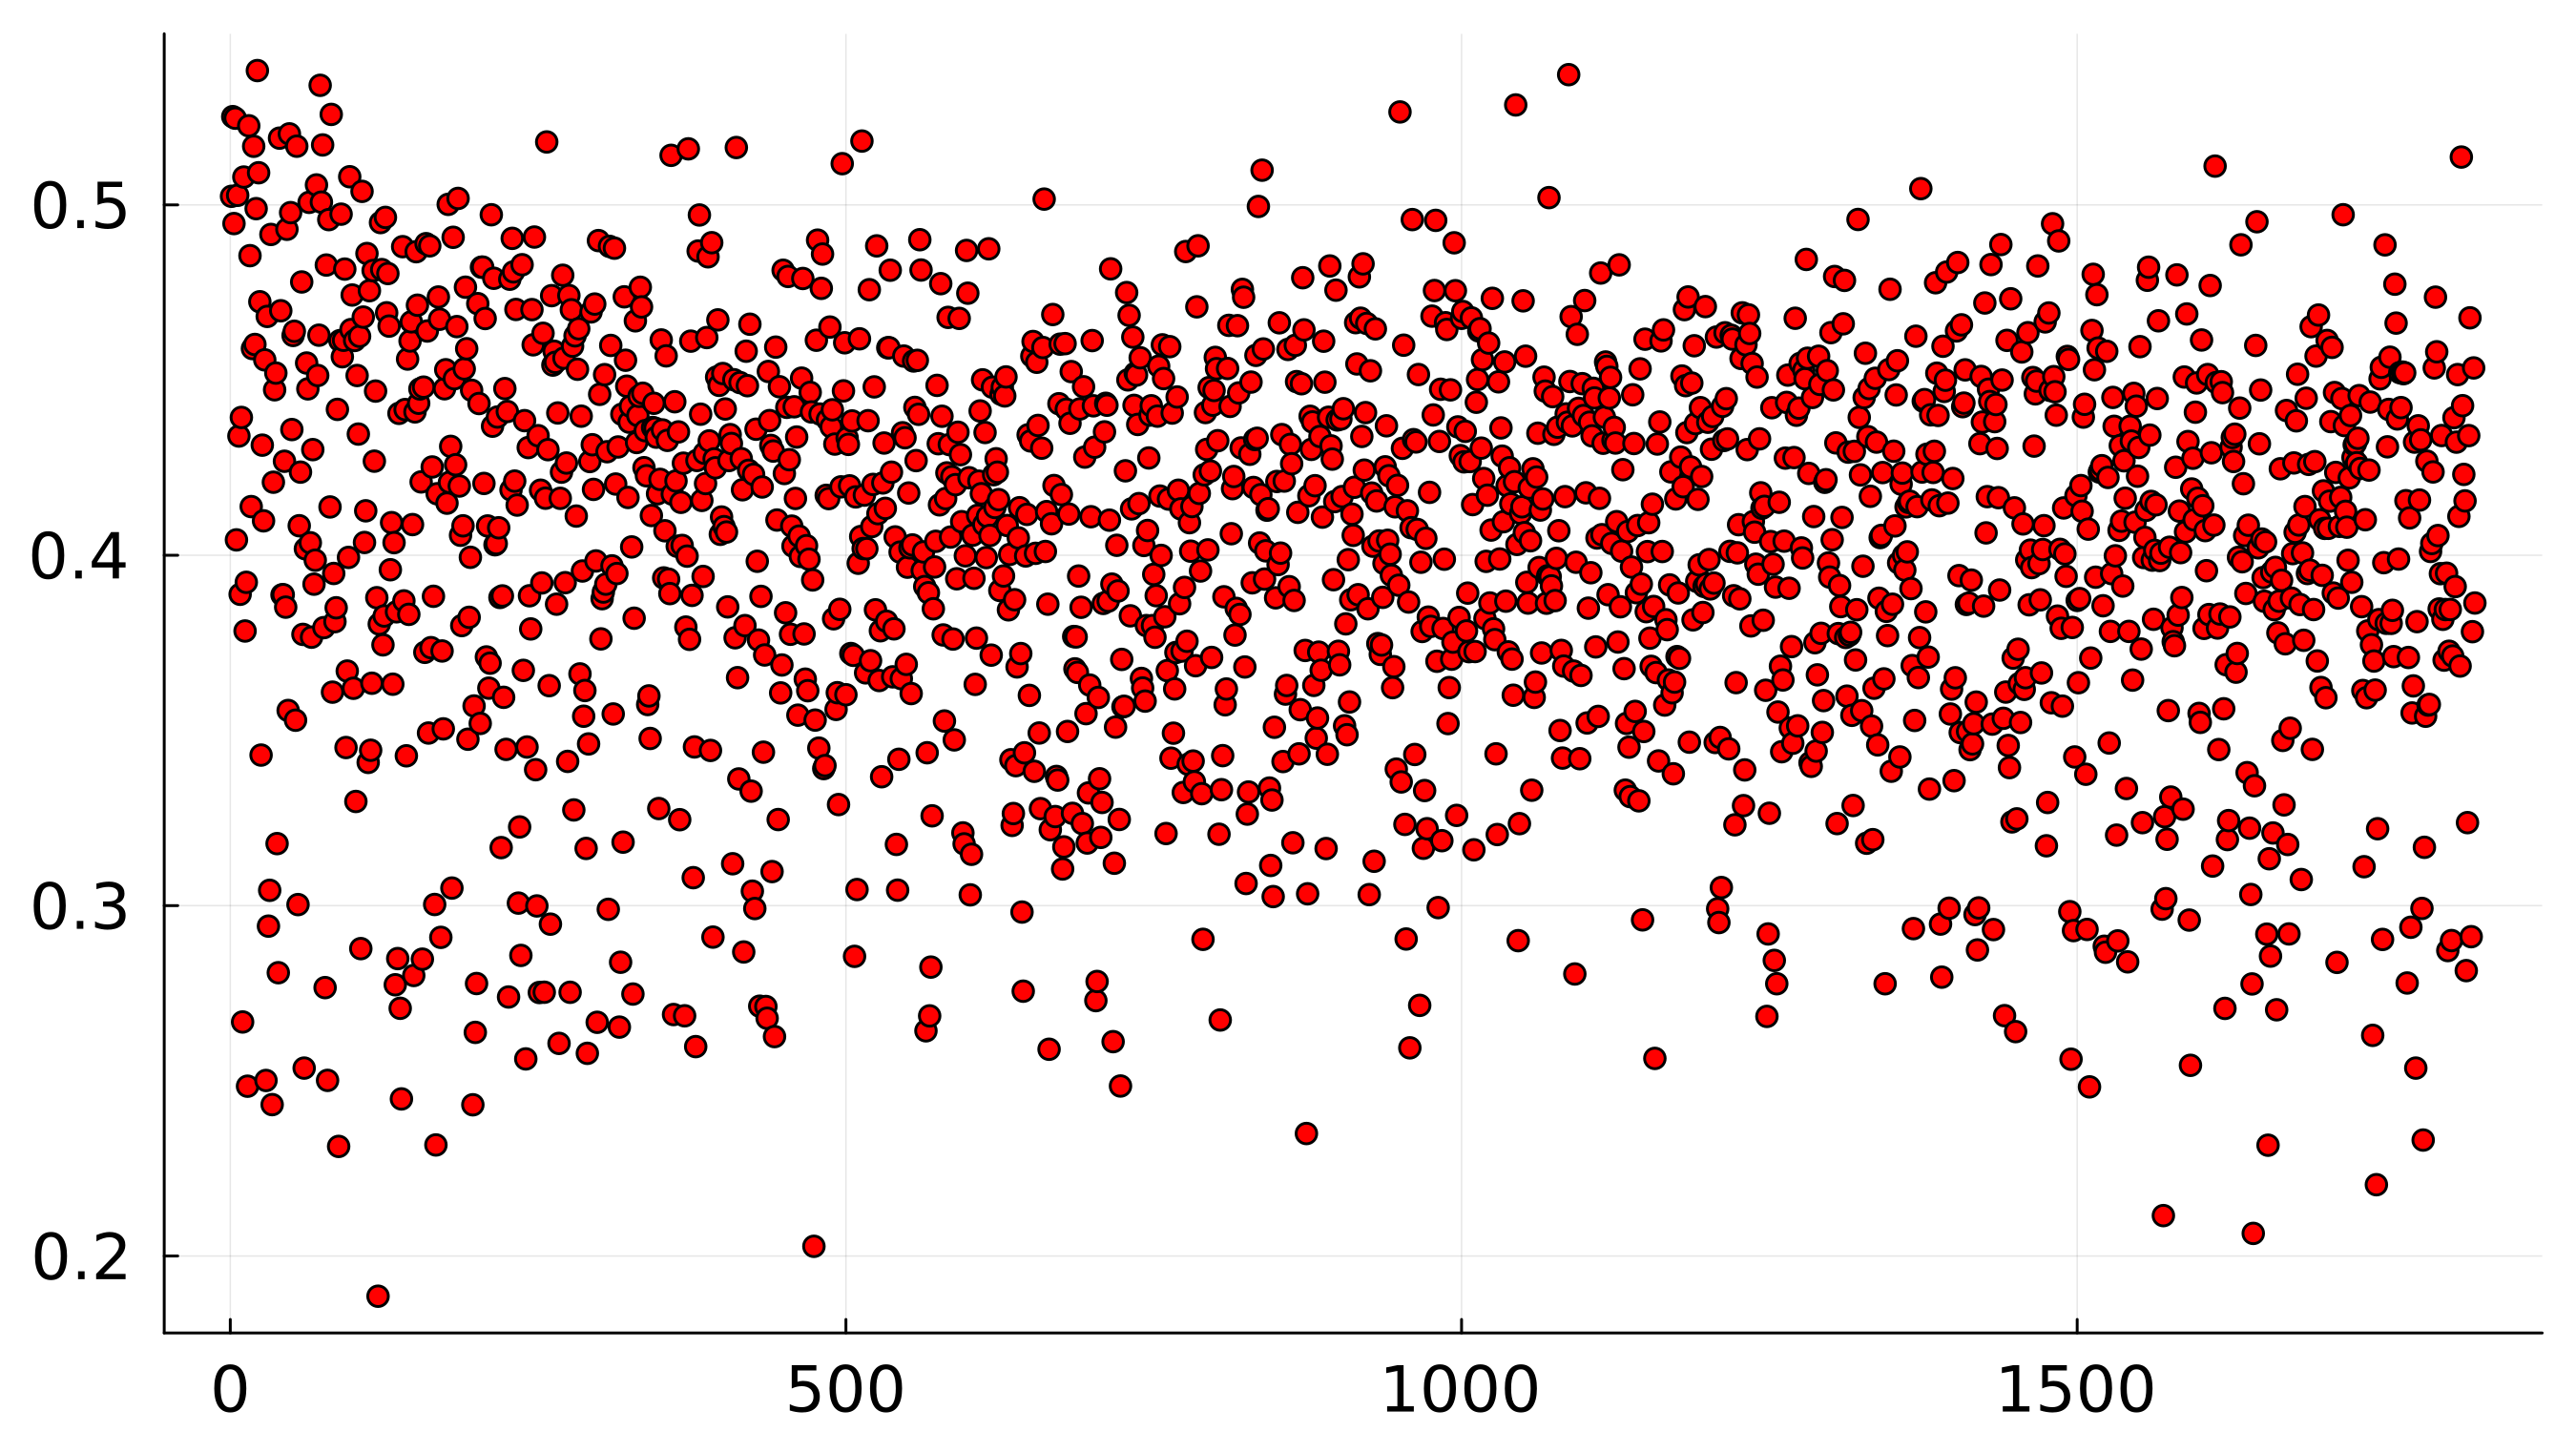
\includegraphics[width=\textwidth]{phalp_bow_esm_learningV}
        \caption{VALs embedded using extended ESM-2 amino acid vectors \textit{via} the bag-of-words embedding method}
        \label{fig:subfig-c}
    \end{subfigure}
    \hfill
    \begin{subfigure}{0.48\textwidth}
        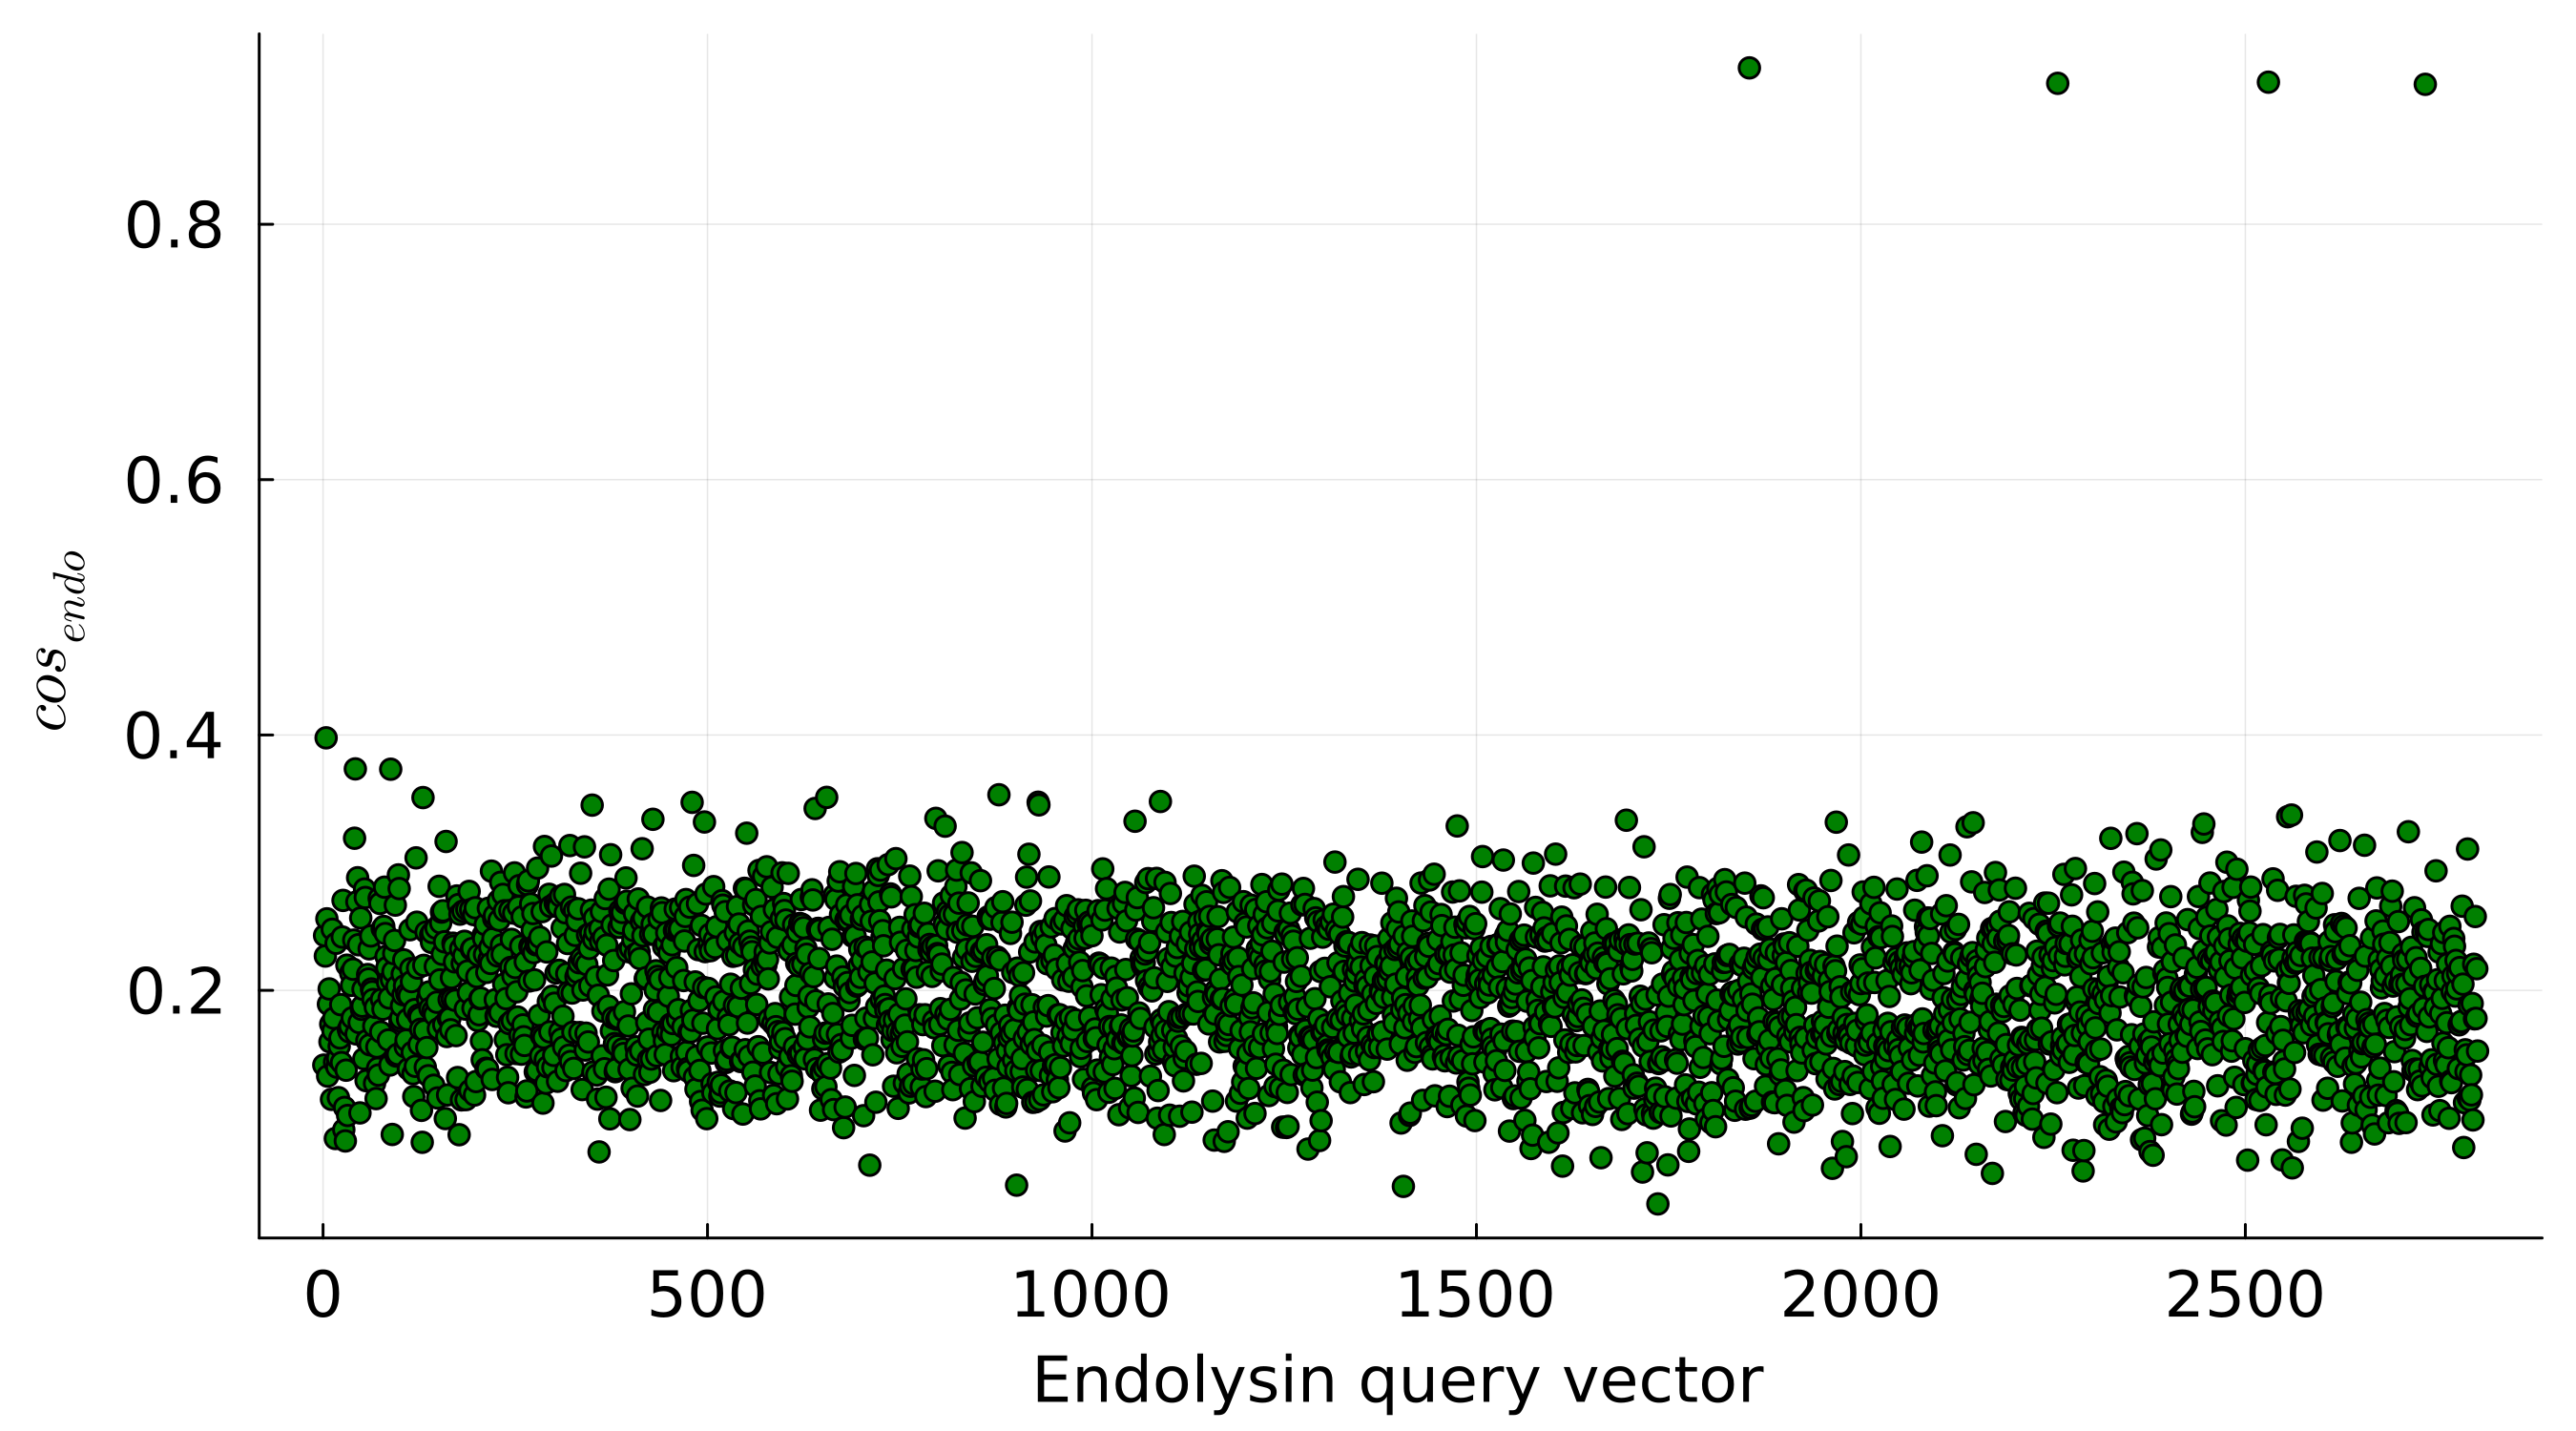
\includegraphics[width=\textwidth]{phalp_bow_esm_learningE}
        \caption{Endolysins embedded using extended ESM-2 amino acid vectors \textit{via} the bag-of-words embedding method}
        \label{fig:subfig-d}
    \end{subfigure}
    
    \begin{subfigure}{0.48\textwidth}
        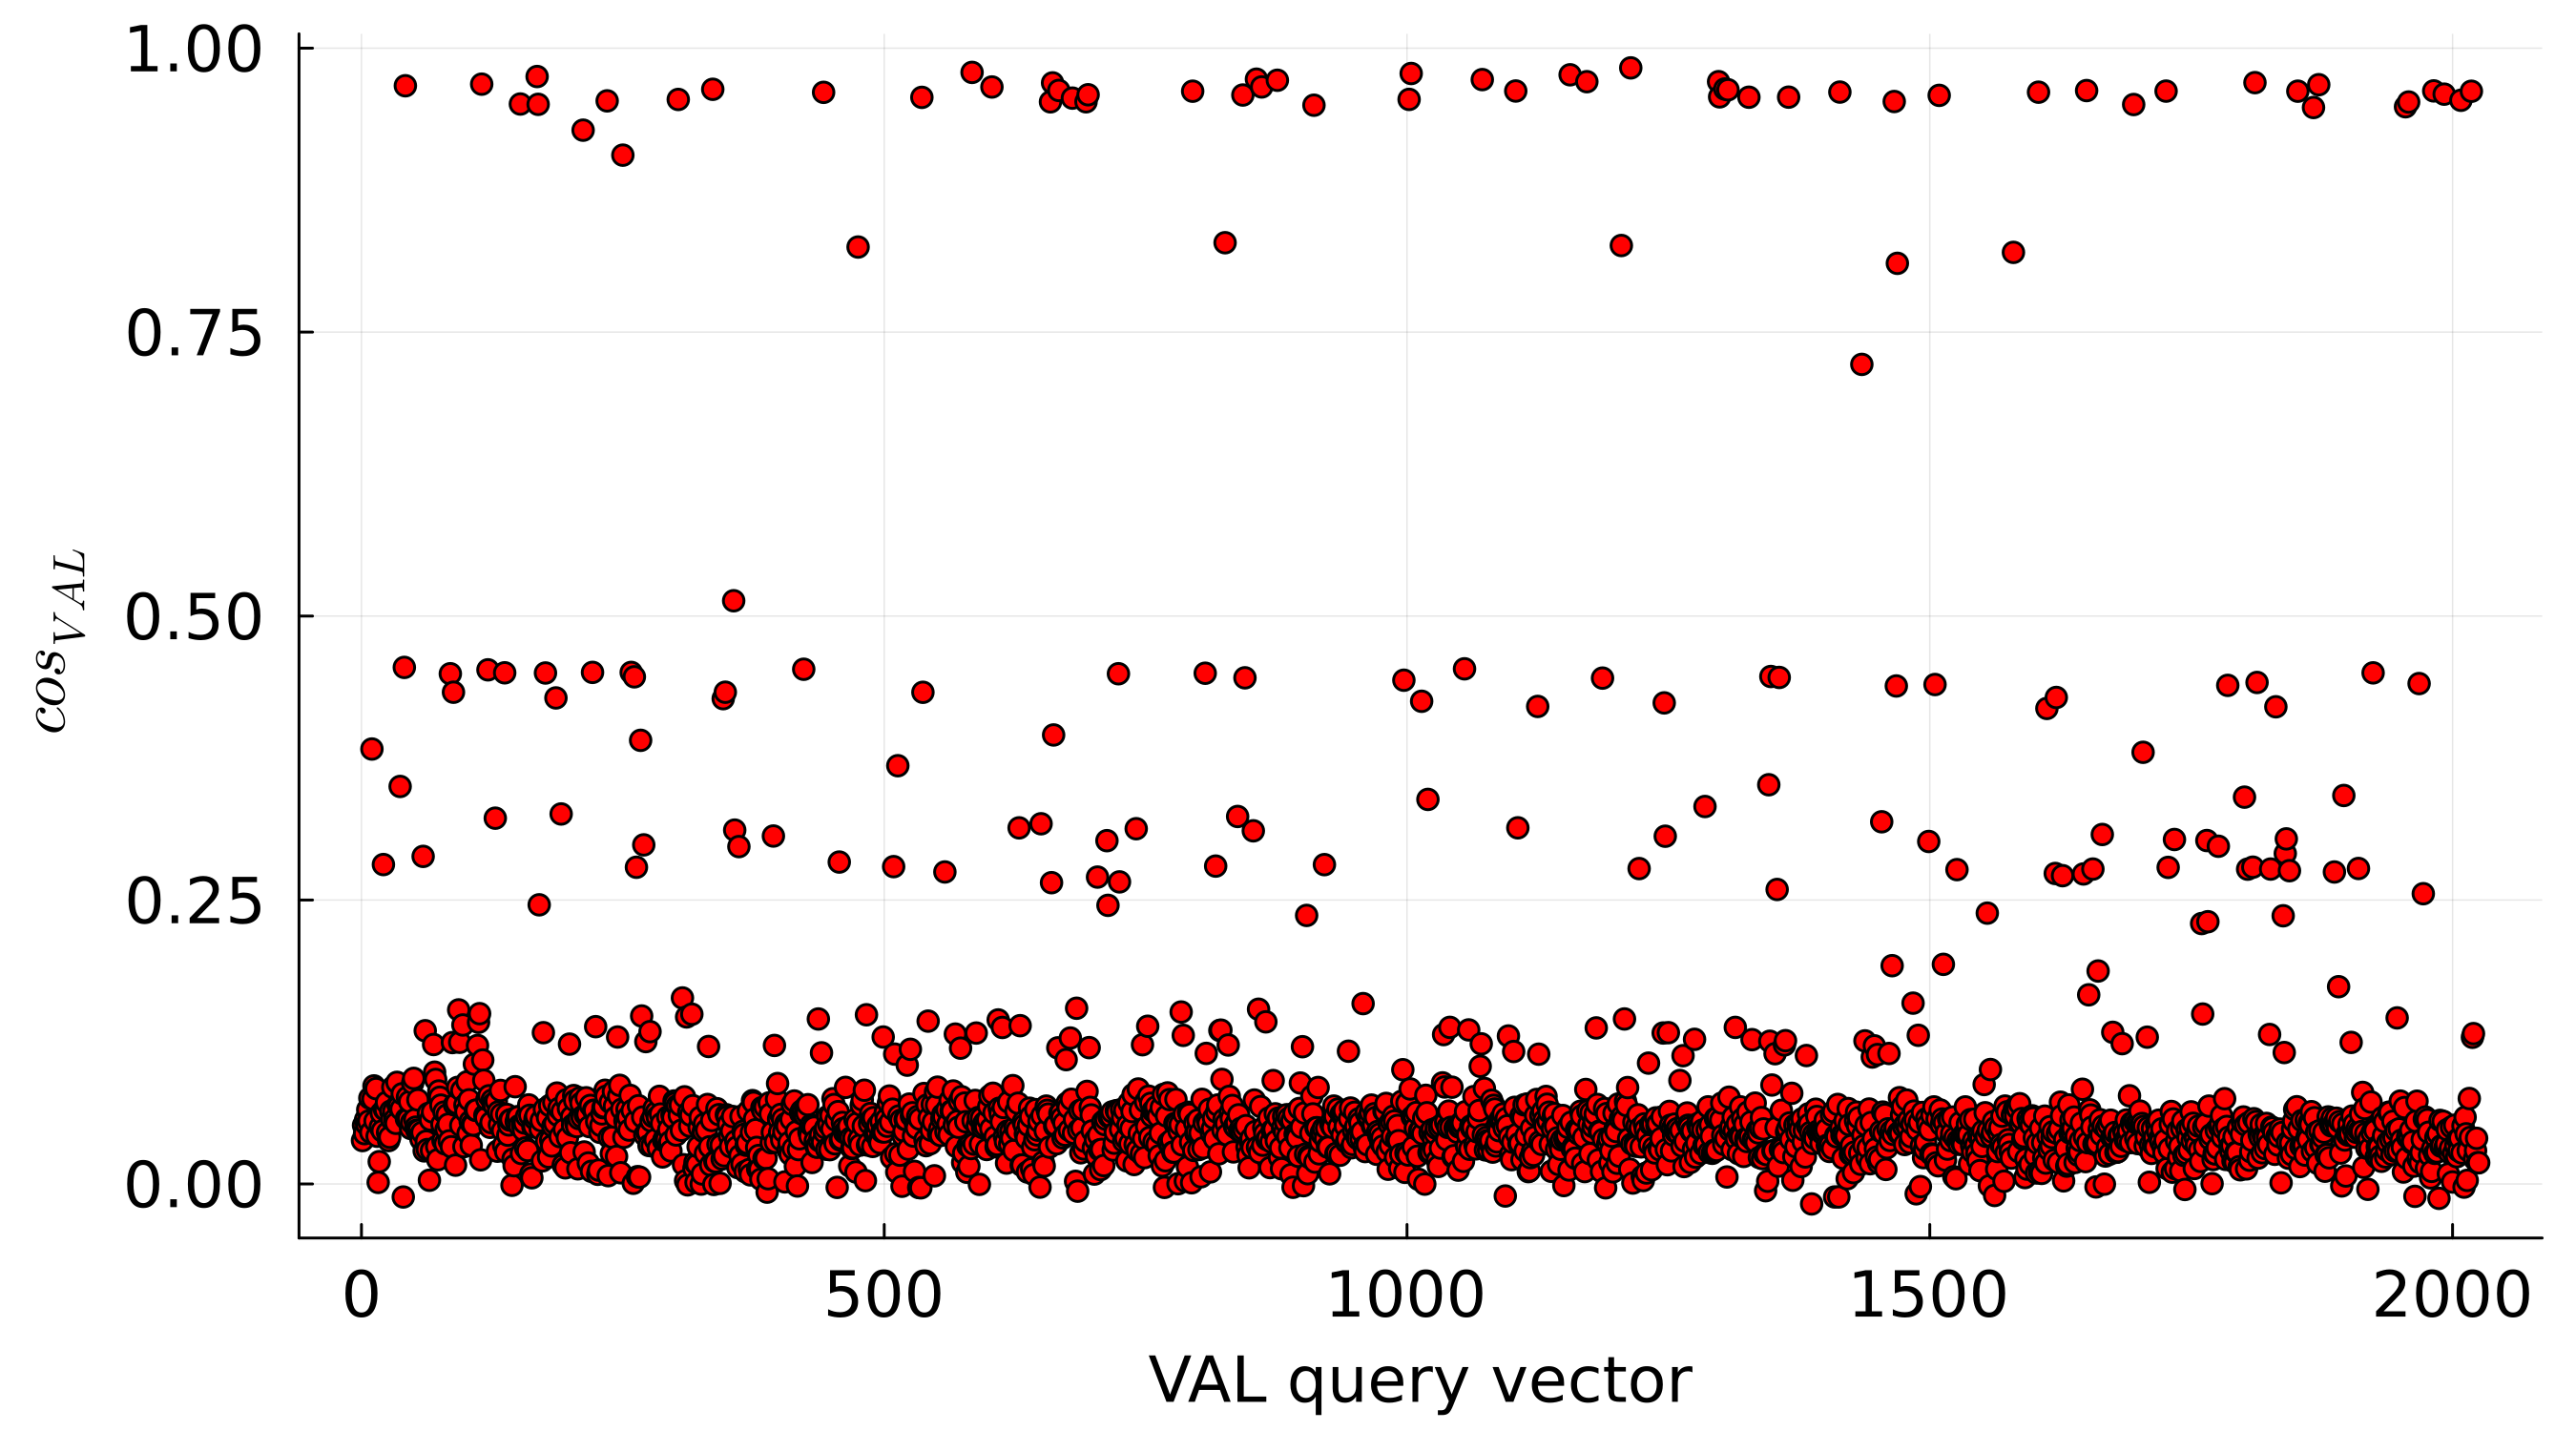
\includegraphics[width=\textwidth]{phalp_cnn_rand_learningV}
        \caption{VALs embedded using using random amino acid vectors \textit{via} the convolutional embedding method}
        \label{fig:subfig-e}
    \end{subfigure}
    \hfill
    \begin{subfigure}{0.48\textwidth}
        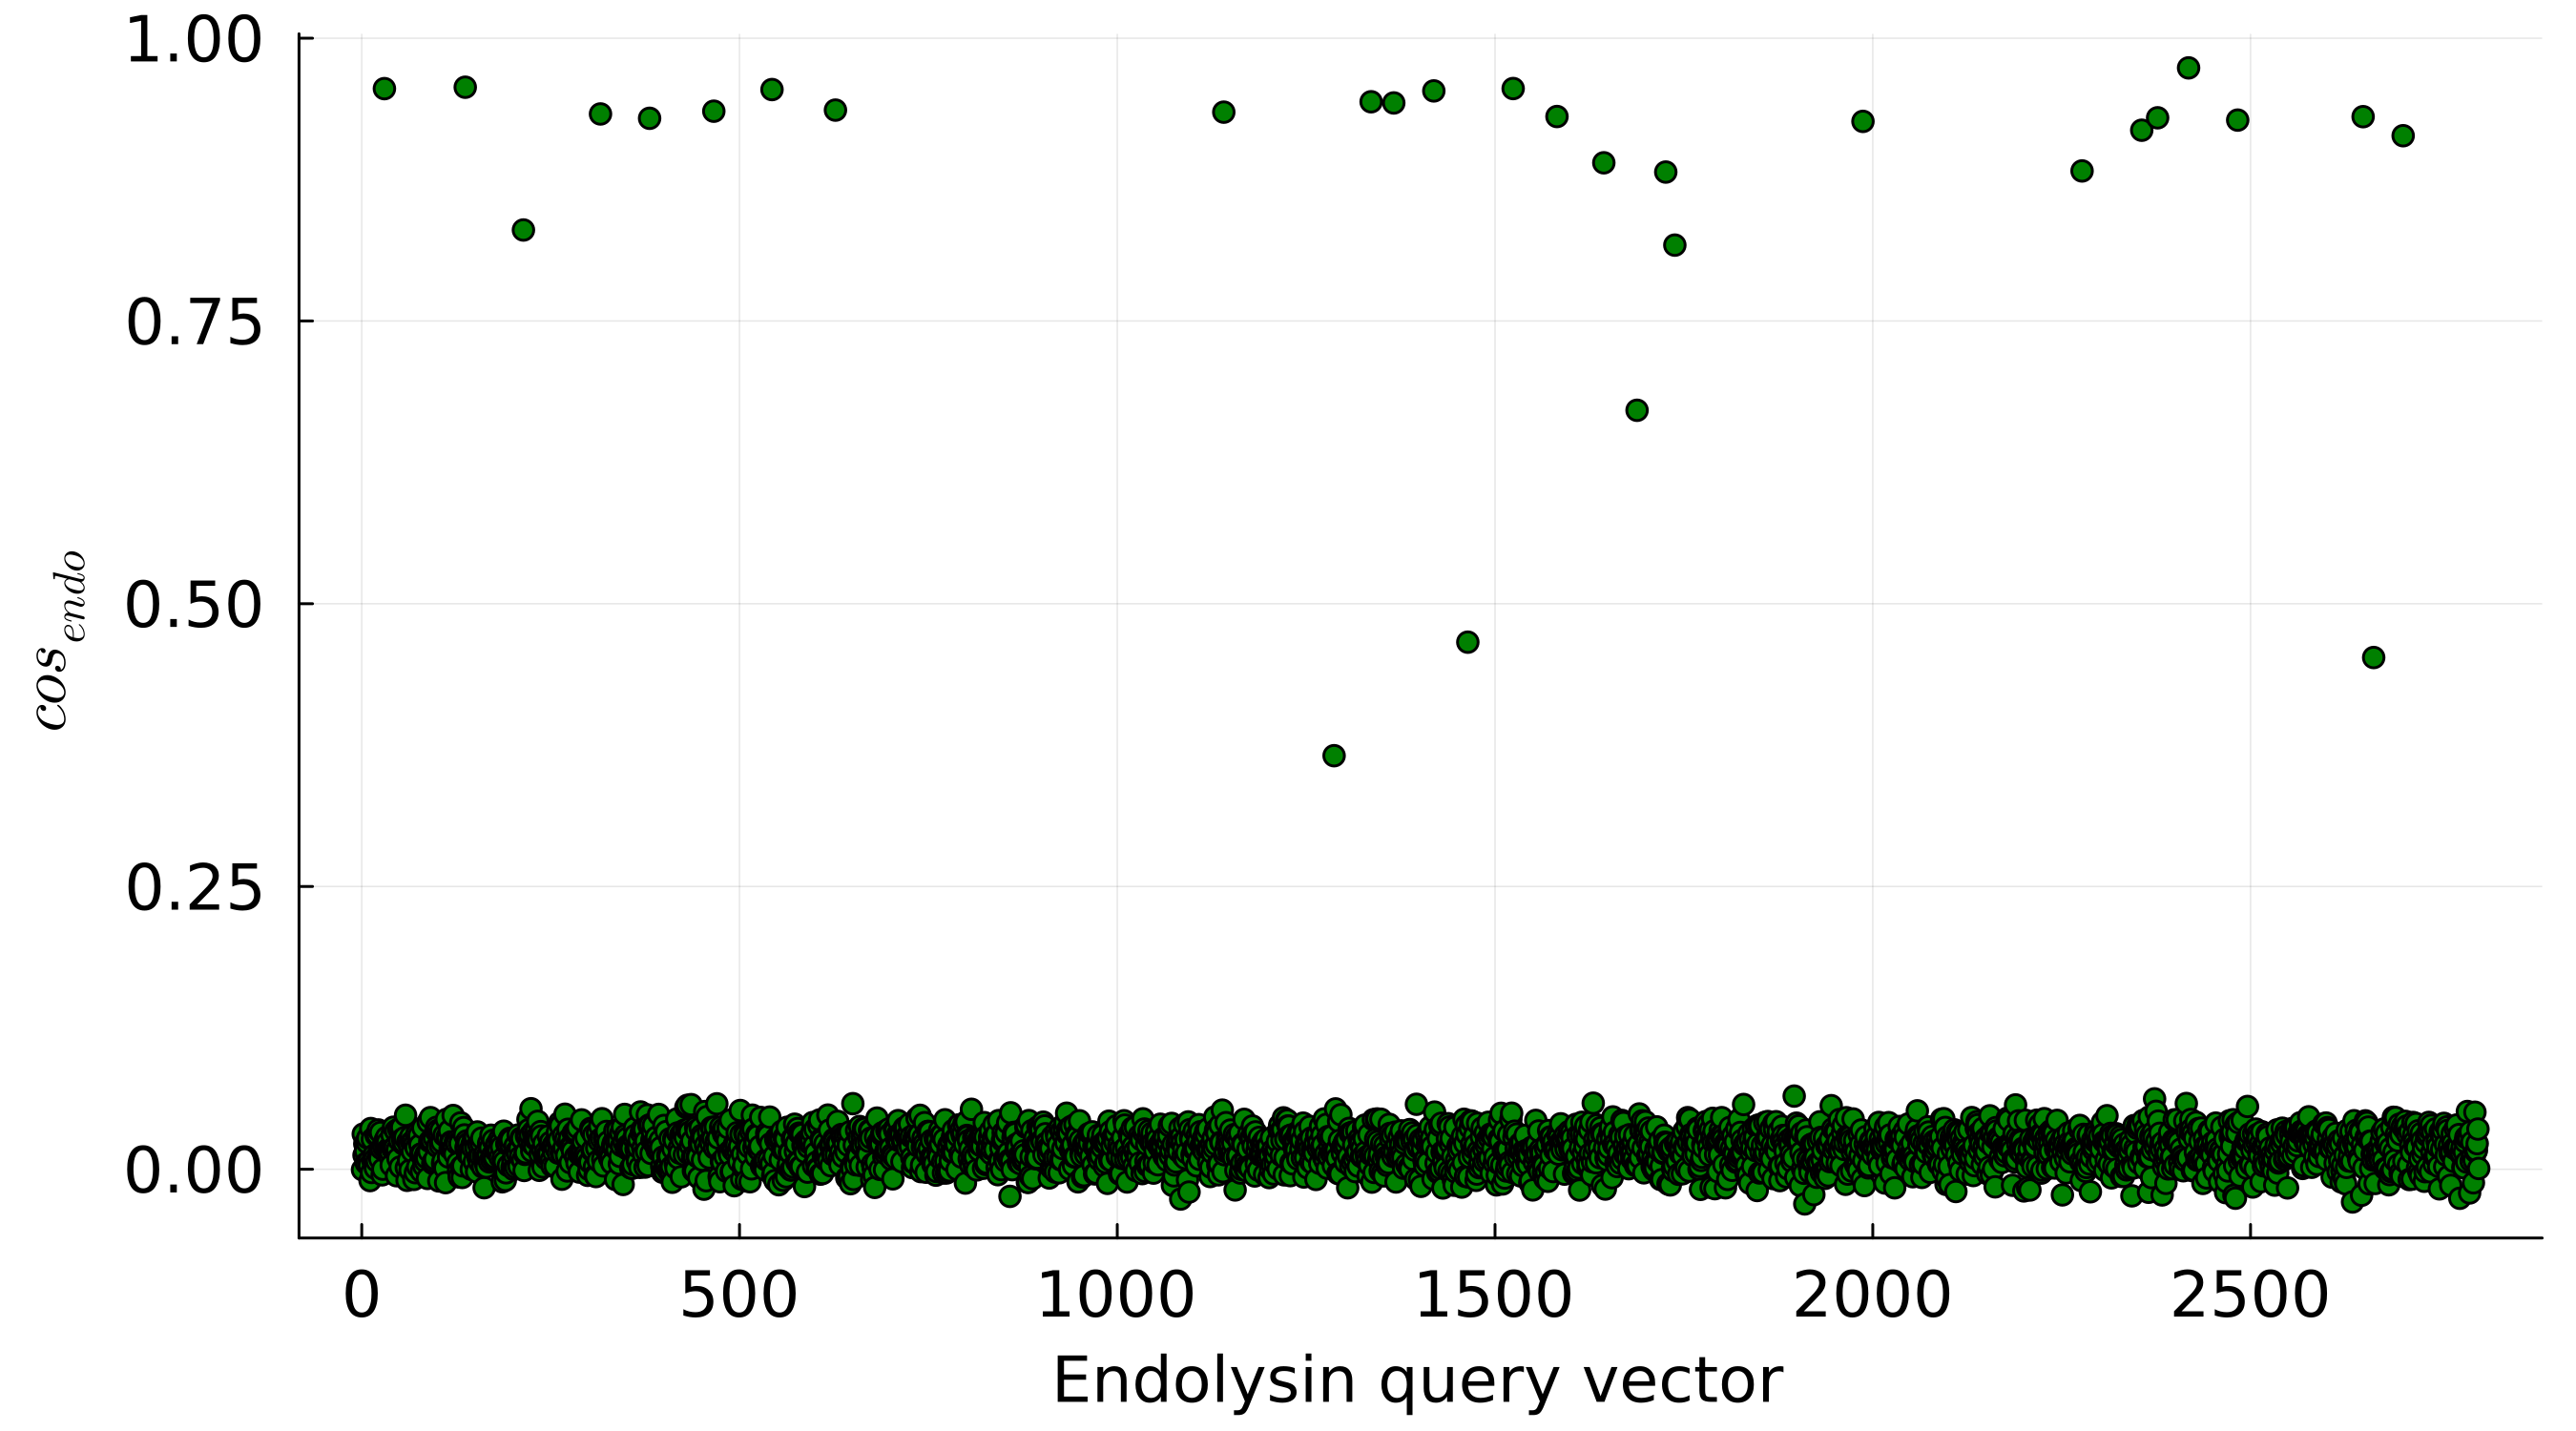
\includegraphics[width=\textwidth]{phalp_cnn_rand_learningE}
        \caption{Endolysins embedded using random amino acid vectors \textit{via} the convolutional embedding method}
        \label{fig:subfig-f}
    \end{subfigure}
    
    \begin{subfigure}{0.48\textwidth}
        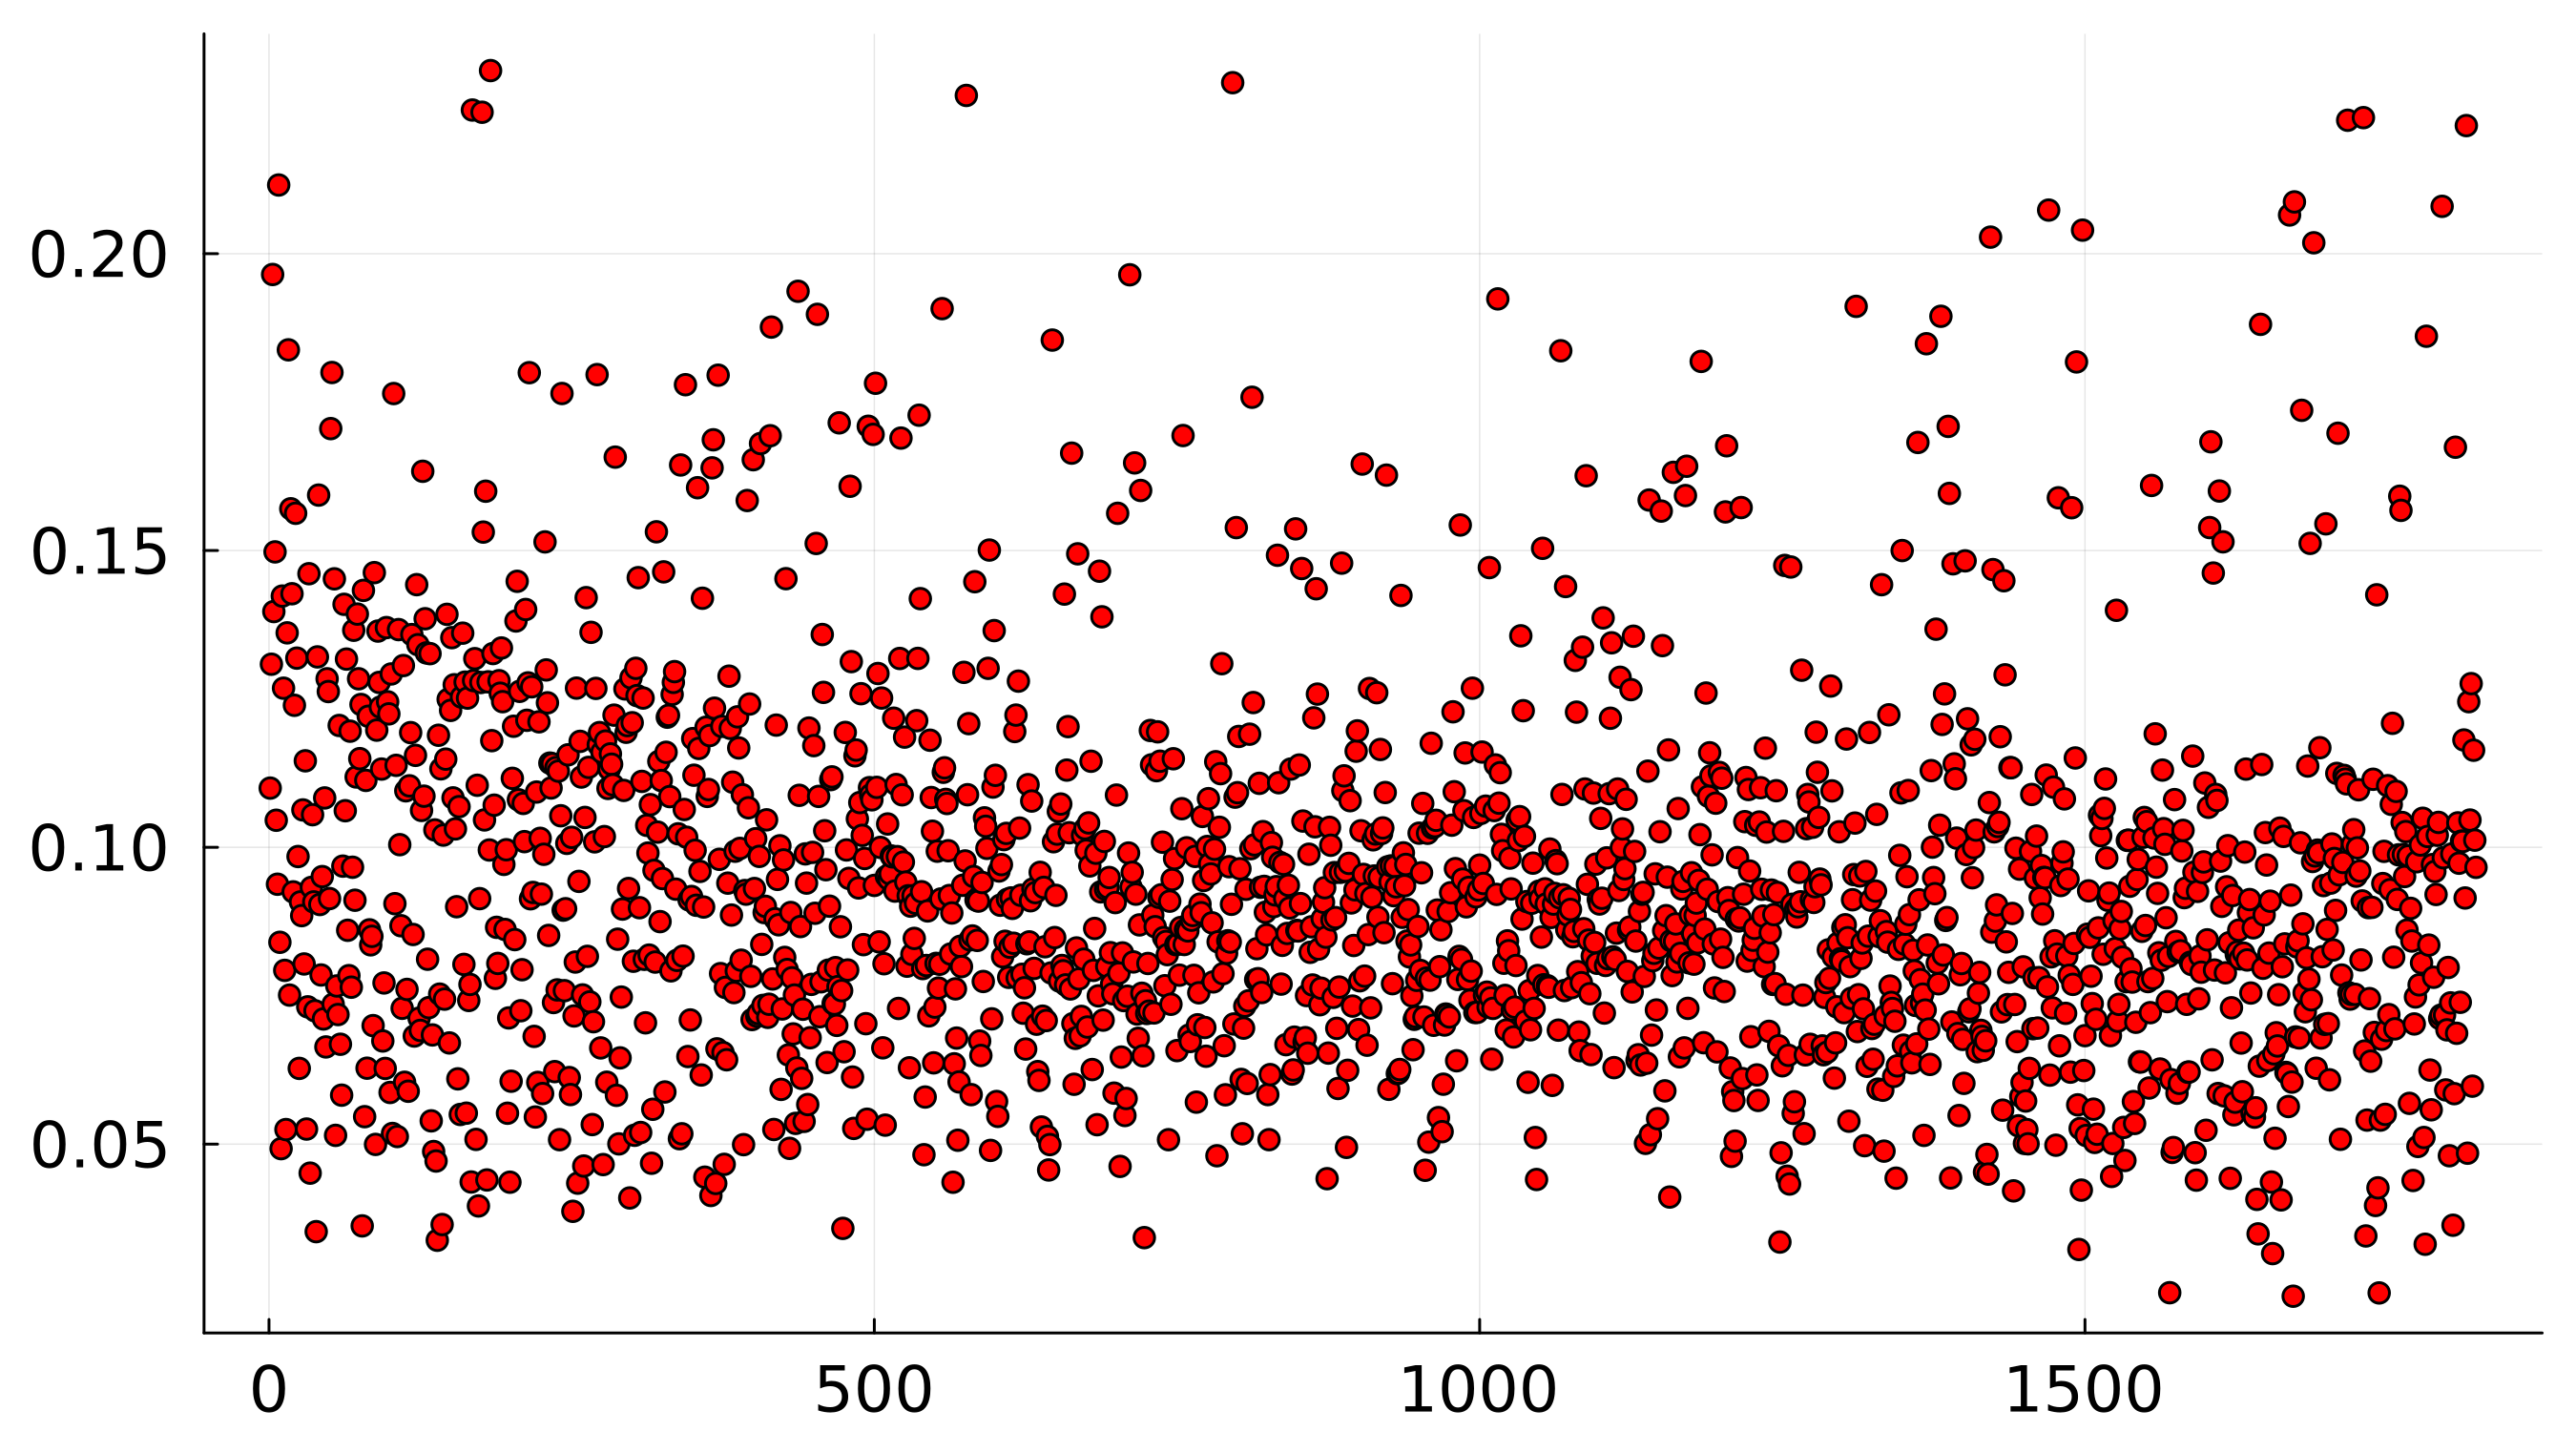
\includegraphics[width=\textwidth]{phalp_cnn_esm_learningV}
        \caption{VALs embedded using extended ESM-2 amino acid vectors \textit{via} the convolutional embedding method}
        \label{fig:subfig-g}
    \end{subfigure}
    \hfill
    \begin{subfigure}{0.48\textwidth}
        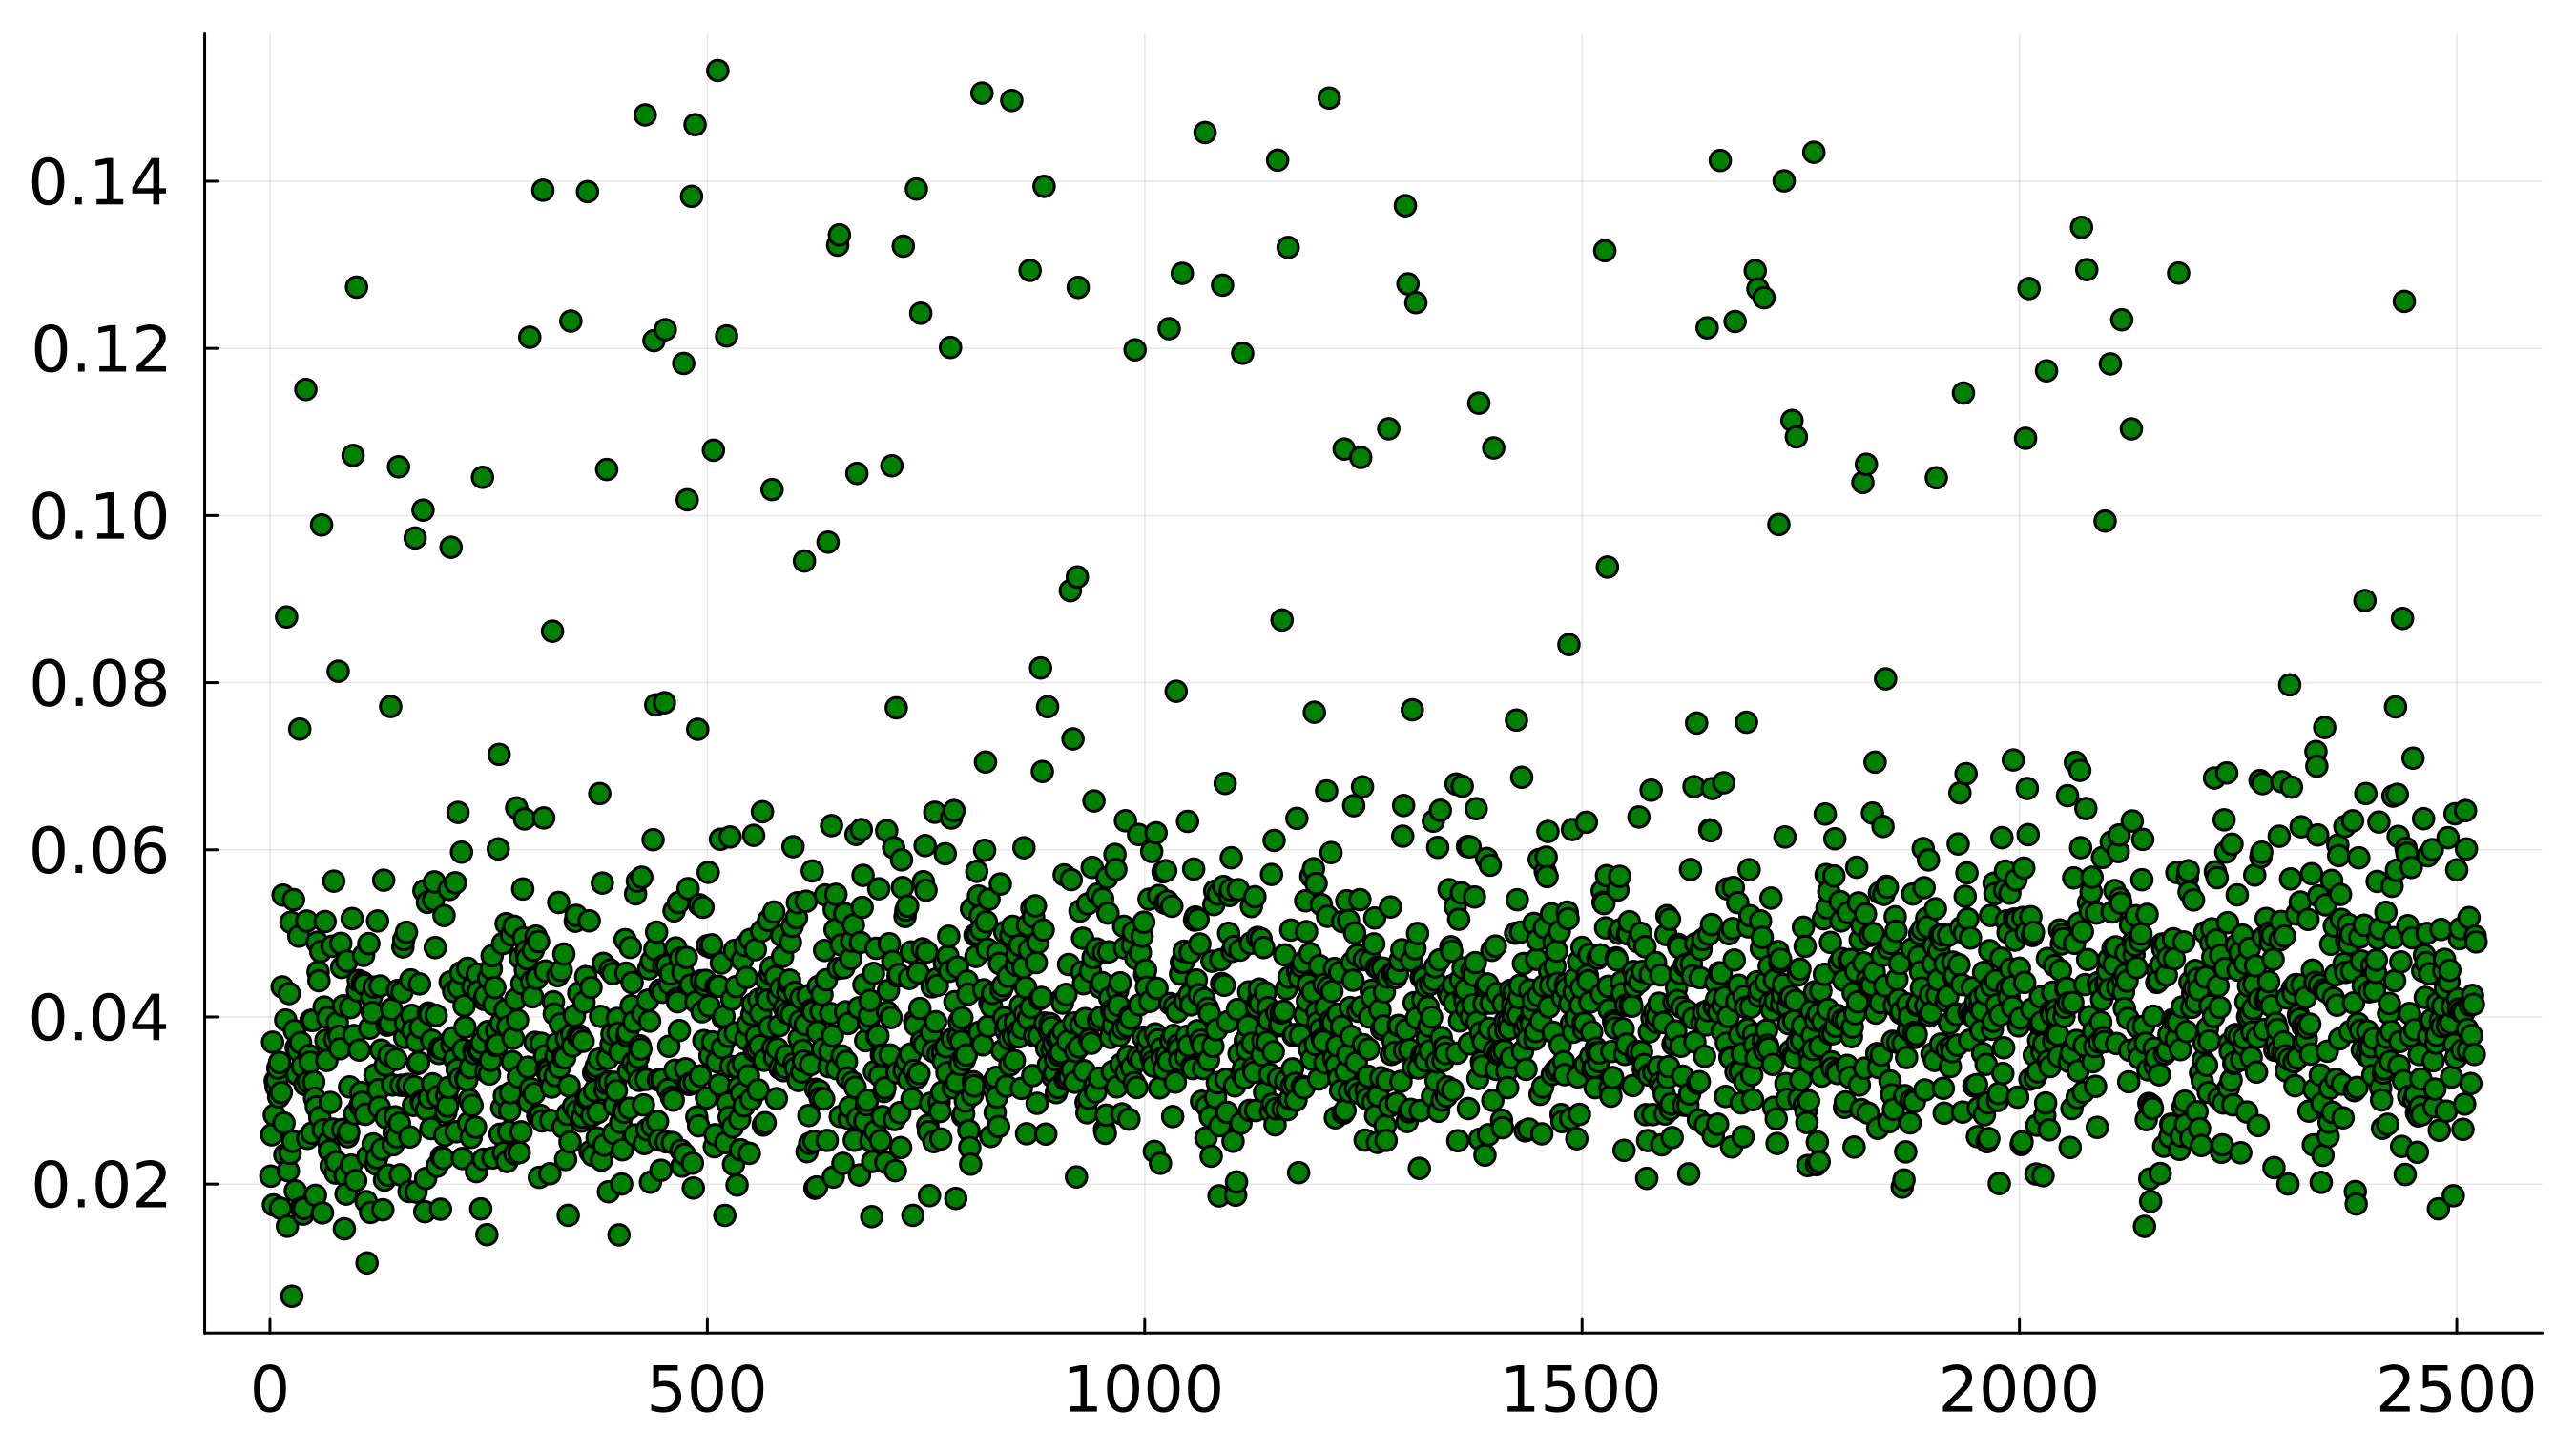
\includegraphics[width=\textwidth]{phalp_cnn_esm_learningE}
        \caption{Endolysins embedded using extended ESM-2 amino acid vectors \textit{via} the convolutional embedding method}
        \label{fig:subfig-h}
    \end{subfigure}
    
    \caption{Average cosine similarity between a query vector and the class vector across the 10 cross validations with OnlineHD single-pass training procedure. Trained using hyperdimensional embeddings from all protein sequences in the PhaLP dataset whose types were manually annotated, red representing VALs and green representing endolysins.}
    \label{fig:main}
\end{figure}

In Figure~\ref{fig:main}, we aim to monitor the two class vectors $\vec{C_{VAL}}$ and $\vec{C_{endo}}$ individually. For each query vector with a known label $l$, we calculate the cosine similarity $cos_{l}$ and average these values across the 10 cross-validation folds. This method allows us to observe the model's adaptation and refinement of its internal representation of the two classes during the training process. The distance between a query vector and a class vector is proportional to the update weight, so we expect the cosine similarities to increase as the model learns.

In this case, the VAL vector updates with relatively consistent weights. This observation, together with Figure~\ref{fig:phalpbowesm}, suggests that virion-associated lysins may have more diverse sequences compared to endolysins. We also notice higher overall similarities between the query vectors and the VAL vector when using the BoW-method with extended ESM-2 vectors, which aligns with this model's superior performance.

The endolysin vector appears to slightly increase its similarity to the query vectors as it trains, with less variation in similarities, indicating that endolysins may have less diverse sequences. As observed with the VAL vectors, the similarities between the query vectors and the endolysin vector are higher when the embeddings are created using the BoW-method with extended ESM-2 vectors.

In Figure~\ref{fig:main3}, we adopt an alternative approach to monitor the training progress of an OnlineHD model. The dataset is divided into training and testing sets, while ensuring stratification is preserved, with the test set comprising 10 \% of the data. The training data is further partitioned into 500 batches, and the model is trained incrementally using these batches. After each batch is processed, the model's performance on the test data is assessed to provide insights into its learning trajectory.

\begin{figure}[h!]
    \centering
    \begin{subfigure}{0.48\textwidth}
        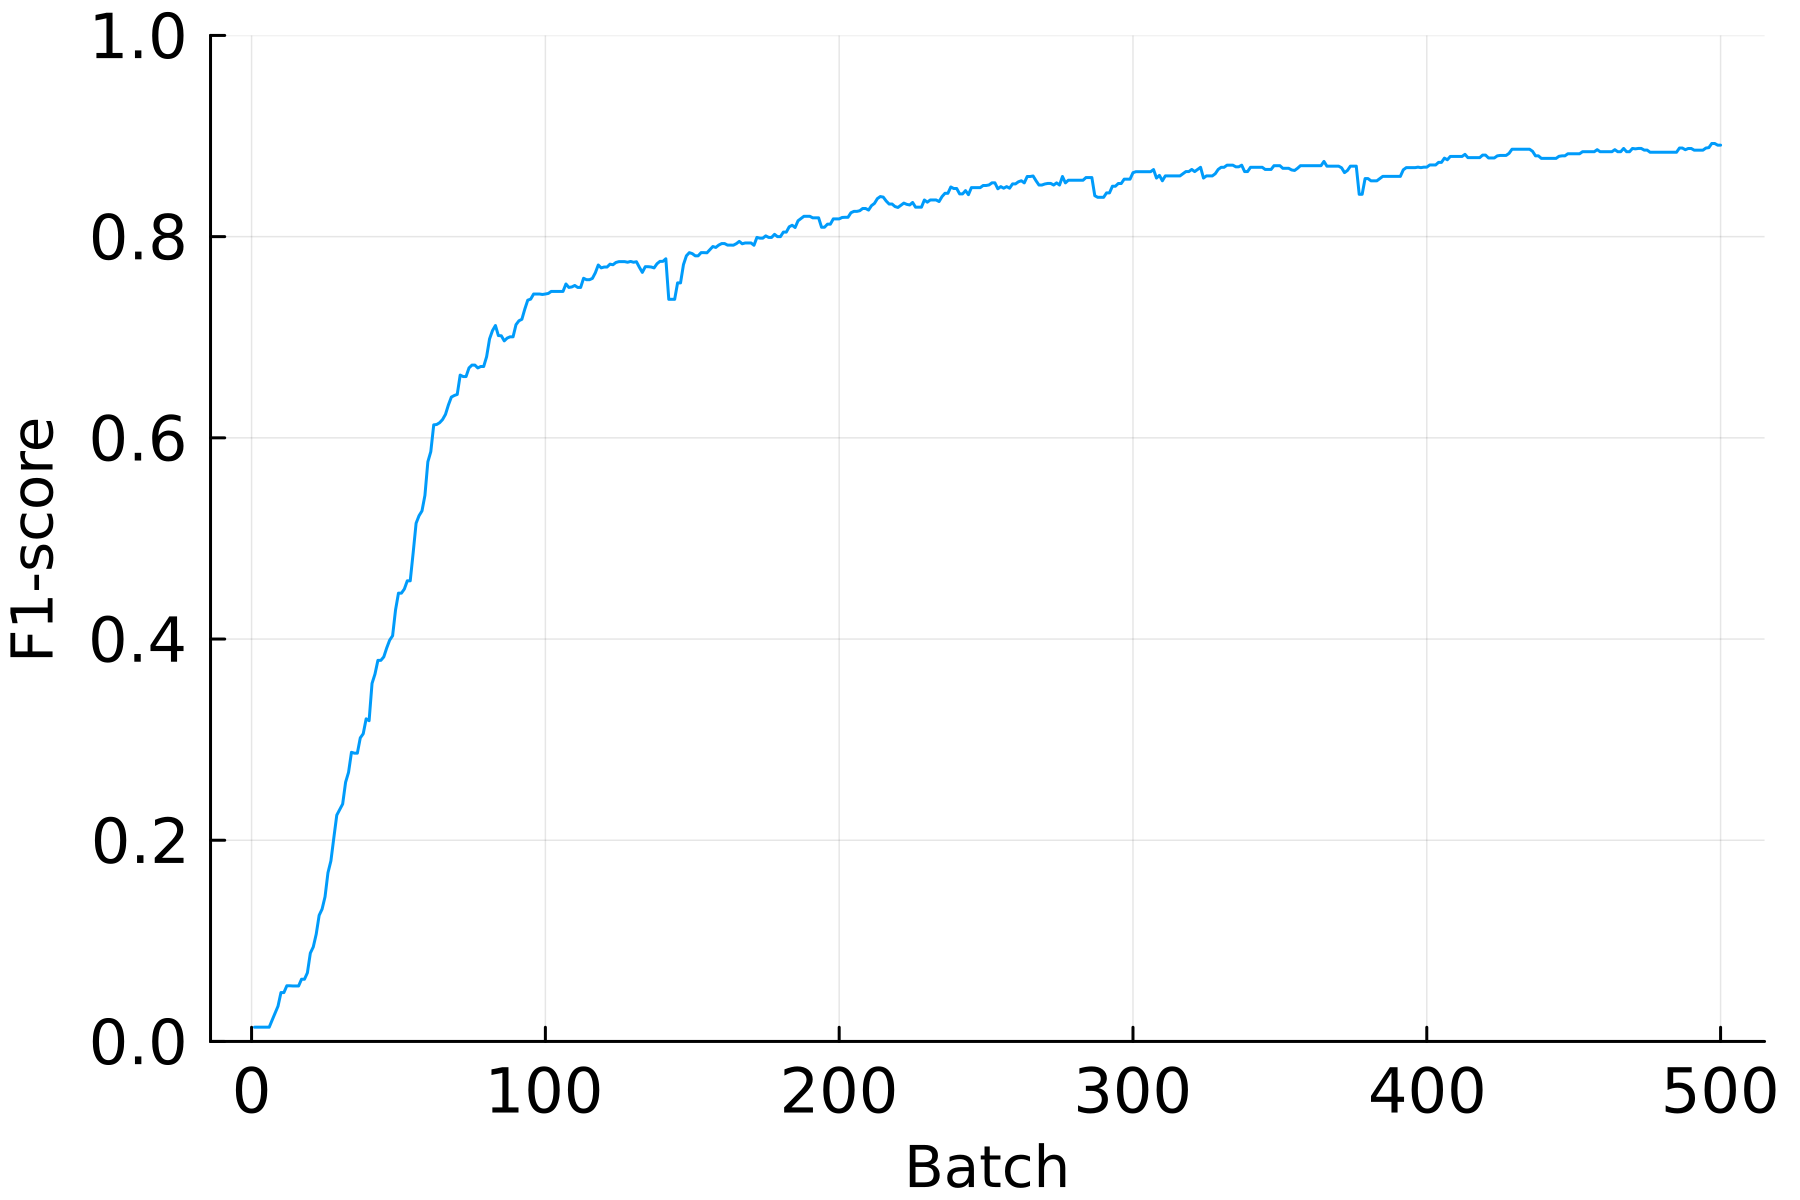
\includegraphics[width=\textwidth]{phalp_bow_rand_score}
        \caption{Embeddings using random amino acid vectors, made \textit{via} the bag-of-words embedding method}
        \label{fig:subfig-a3}
    \end{subfigure}
    \hfill
    \begin{subfigure}{0.48\textwidth}
        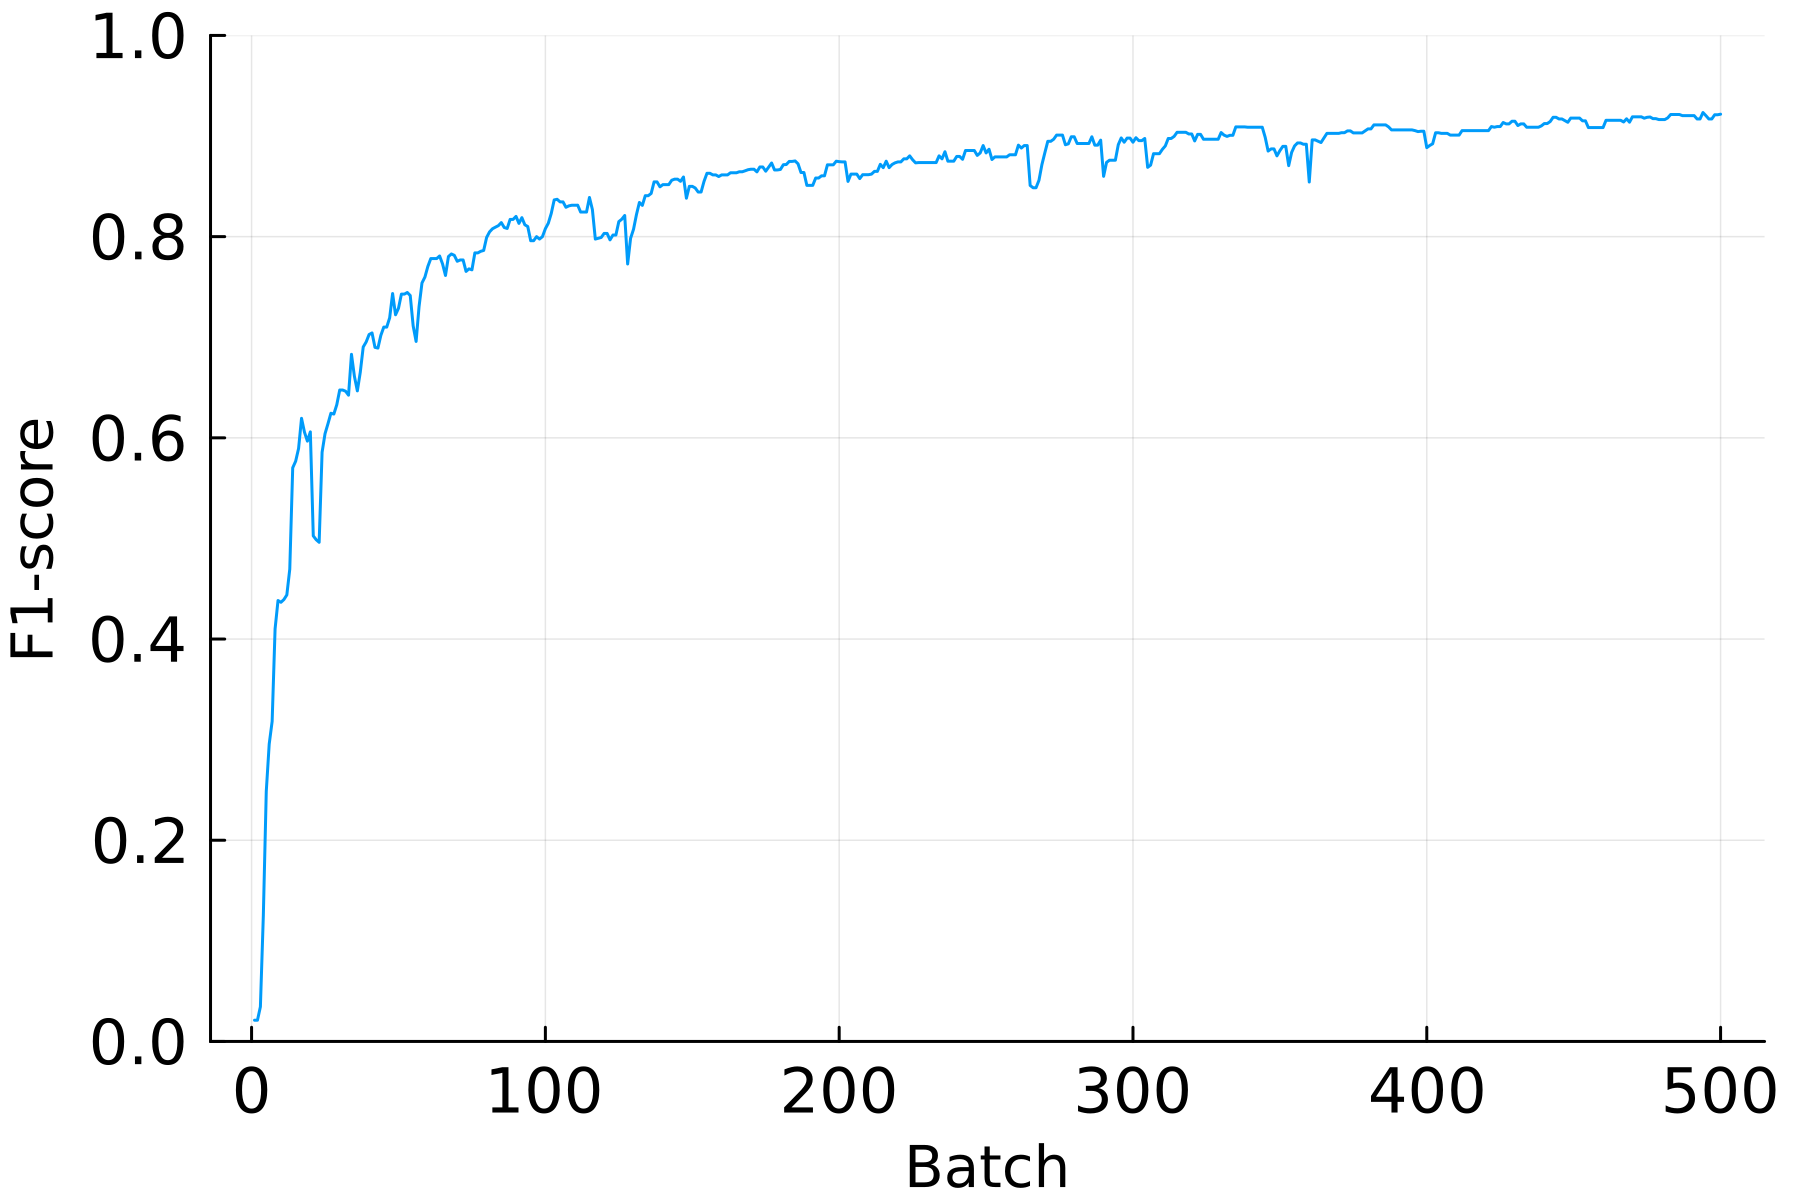
\includegraphics[width=\textwidth]{phalp_bow_esm_score}
        \caption{Embeddings using extended ESM-2 amino acid vectors, made \textit{via} the bag-of-words embedding method}
        \label{fig:subfig-b3}
    \end{subfigure}
    
    \begin{subfigure}{0.48\textwidth}
        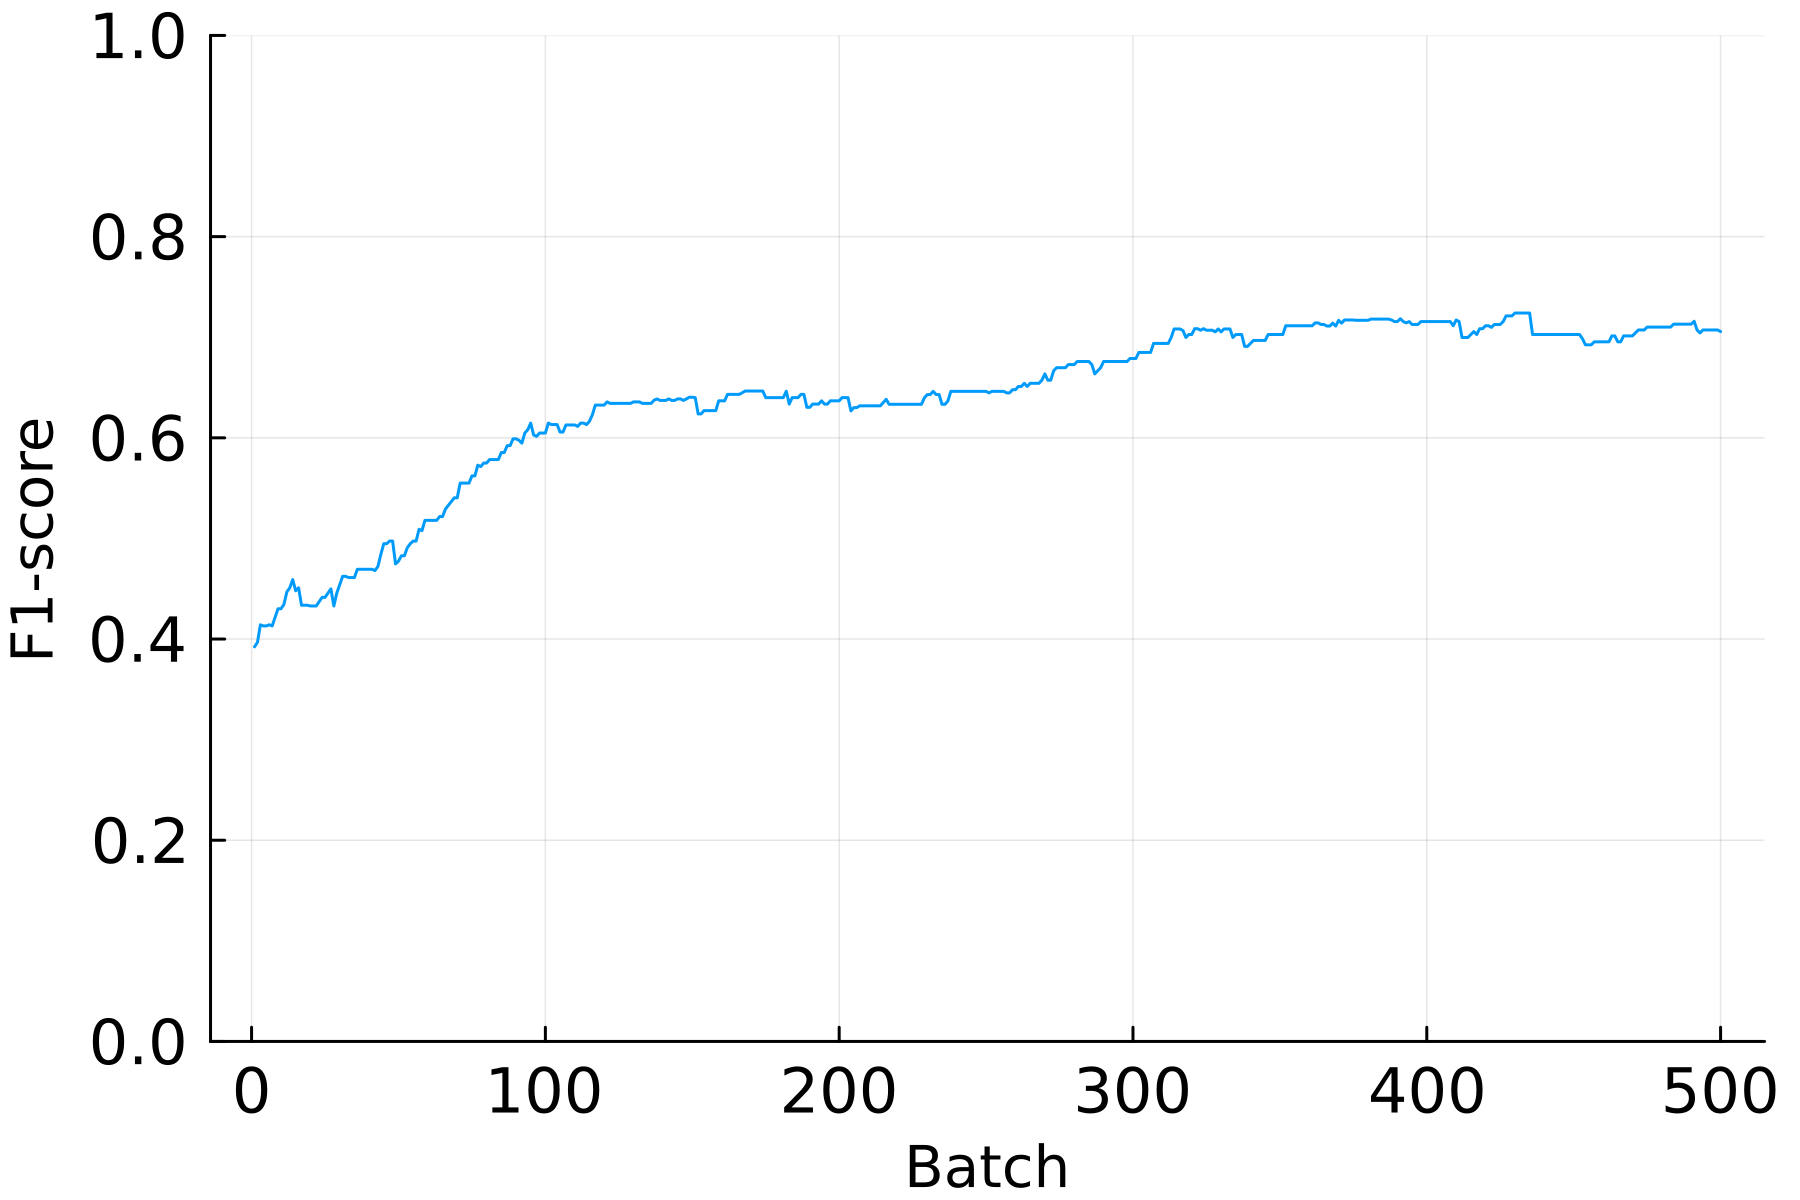
\includegraphics[width=\textwidth]{phalp_cnn_rand_score}
        \caption{Embeddings using random amino acid vectors, made \textit{via} the convolutional embedding method}
        \label{fig:subfig-c3}
    \end{subfigure}
    \hfill
    \begin{subfigure}{0.48\textwidth}
        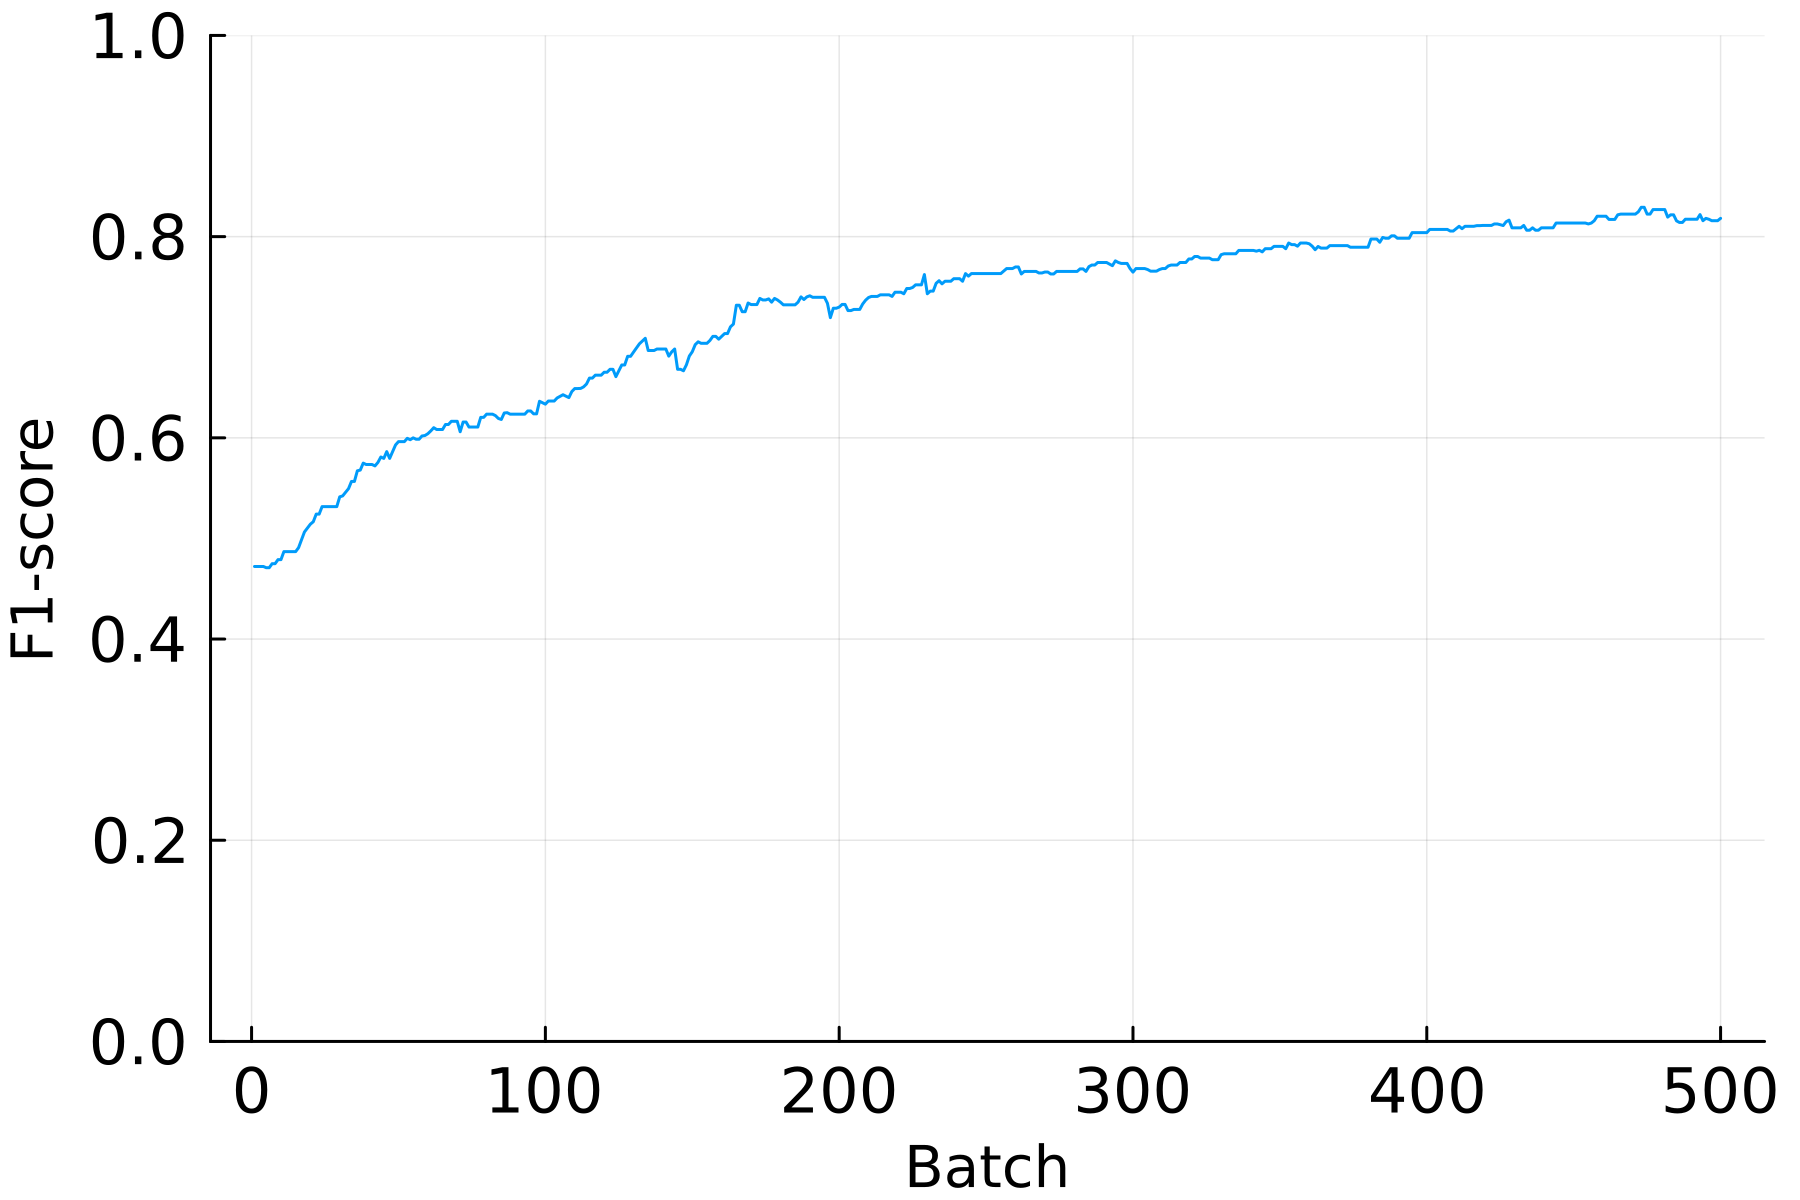
\includegraphics[width=\textwidth]{phalp_cnn_esm_score}
        \caption{Embeddings using extended ESM-2 acid vectors, made \textit{via} the convolutional embedding method}
        \label{fig:subfig-d3}
    \end{subfigure}
    \caption{The F1-score of the OnlineHD single-pass model with a validation set throughout its training procedure. Trained in batches using several kinds of hyperdimensional embeddings from all protein sequences in the PhaLP dataset whose types were manually annotated.}
    \label{fig:main3}
\end{figure}

Upon initial observation, it is apparent that the models trained with embeddings generated using the convolutional method exhibit superior performance from the outset. This higher starting point might be partially attributed to the random initialization of the model. However, a common characteristic observed across all models is that their performance tends to stagnate after approximately 100 batches, which corresponds to roughly 870 sequences in our case. This observation suggests that hyperdimensional computing-based classification methods may exhibit promising performance and effectively capture essential information, even after being exposed to just a small fraction of the training data, which is an intriguing finding for further exploration.